\documentclass{thesis}

% Writing Tips ================================================================
% Your research question should always be kept in mind. Write with it.
% https://moodle.gla.ac.uk/pluginfile.php/2676039/mod_resource/content/1/PRISMA%20statement.pdf
% https://moodle.gla.ac.uk/course/view.php?id=12843&section=7

% Style Guide =================================================================
% https://moodle.gla.ac.uk/pluginfile.php/4294369/mod_resource/content/1/ODL%20Project%20Style%20Guide.pdf
% The page limit is 25-30 for main content.

\usepackage{pdfpages}

\begin{document}

% Metadata ====================================================================

\title{Regressing Litter on Deprivation in Glasgow City with Object Detection}
\author{Gary Blackwood}
\date{\today}
\maketitle

% Abstract ====================================================================
% https://www.scribbr.com/dissertation/abstract/
% https://www.discoverphds.com/advice/doing/abstract-for-a-dissertation-or-thesis
% https://mantex.co.uk/how-to-write-a-thesis-abstract/

\begin{abstract}
    \todo{Abstract -- An executive summary of roughly 500 words.}
\end{abstract}

% Acknowledgements ============================================================
% https://www.discoverphds.com/advice/doing/acknowledgements-for-thesis-and-dissertations
% https://prothesiswriter.com/blog/how-to-write-an-acknowledgement-for-a-thesis

\chapter*{Acknowledgements}
\todo{Acknowledge those that helped me throughout the project.}

% List of Figures and List of Tables ==========================================

\listoffigures
\listoftables

%==============================================================================

\tableofcontents

% Introduction ================================================================
% Background to research
% Research question
% Research aims
% Scope of research
% Importance of research
% Assumptions

\chapter{Introduction}
\pagenumbering{arabic} % Don't remove this!

The Scottish city of Glasgow was home to the 26th UN Climate Change Conference during the month of November 2021. Known as COP26, the gathering of world leaders, with thousands of delegates and diplomats in tow, was thought to be humanities last chance to commit to the changes necessary to keep global temperatures from rising past the limit of 1.5 degrees Celsius above pre-industrial levels. Breaking through this threshold would see catastrophic outcomes such as the increased intensity and frequency of droughts and floods\cite{impacts-of-15}.

This rightful focus on the global climate emergency overshadowed another environmental problem. One which, for Glasgow City at least, is at its worst state in years\cite{tackle-litter} -- the amount of litter on its streets.

According to a recent study by Keep Scotland Beautiful, the issue of litter creates the most public outcry\cite{household-survey-2019} and is an important indicator of overall environmental quality. Unfortunately, the study found that since 2016, the state of our public spaces has been in decline. None more so than in the most deprived areas of the country where the number of significantly littered sites has more than doubled since 2014.

Littering behaviour is strongly affected by the social context in which it occurs\cite{littering-behaviour}. Research by Zero Waste Scotland found that in addition to personal factors such as age and gender, social factors influenced the prevalence of litter. If individuals in an area deem it socially acceptable, it is more likely to occur. 

Why is there more litter in the most deprived areas? The socioeconomic problems that come with deprivation may be the answer. If the local population have more pressing troubles to worry about, they may care less about the environmental impacts of litter.

The Scottish Government seeks to understand the circumstances  surrounding deprived communities in order to make effective policy making decisions. If there are links between deprivation and littering, there may be the potential for the improvement of one issue to improve the other. Tackling litter by creating a fairer society is an exciting thought, but first we must discover the links between litter and deprivation.

This study aimed to identify the relationship between the key indicators of deprivation in areas of Glasgow City and the amount of litter on its streets. To this end, the Poisson and Negative Binomial regression models for count data were employed. The ambition was to discover areas of focus that could reduce littering if improved.

Secondary to this aspiration, it was of interest to discover if an automated approach to counting litter on a city scale could be achieved using deep learning object detection methods. Thus far, local organisations have had to perform manual audits to collect such data. Any improvement to this process would be a welcome step towards a cleaner world.

% Literature Review ===========================================================
% https://moodle.gla.ac.uk/mod/resource/view.php?id=841188
% demonstrates a familiarity with a body of knowledge and establishes the credibility of your work;
% summarises prior research and says how your project is linked to it;
% integrates and summarises what is known about a subject;
% demonstrates that you have learnt from others and that your research is a starting point for new ideas.

\chapter{Literature Review}

\section{Object Detection}

\subsection{CNN}

Convolutional Neural Network object detectors use supervised learning and generally consist of two components; a CNN-based backbone that is used for feature extraction, and a head that is used to predict the class and bounding box for an object. In recent years, state-of-art models have begun to insert layers in-between the backbone and head to form a third component known as the neck.

Existing Backbones are typically used for their proven feature extraction capabilities on classification problems. Rather than redesign custom networks, researchers will fine-tune the backbone to increase its suitability to the task at hand. Often used backbones include ResNet, VGG, and CSPDarknet53\cite{zhu2021tphyolov5}.

The purpose of the neck is to improve upon the features provided by the backbone. Usually consisting of several bottom-up and top-down paths, the neck reprocesses the backbone's features at different stages with the goal of aggregating them in preparation for the detection in the head.

The responsibility of detecting the location and category of an object falls upon the head. It takes the features extracted from the preceding layer's classification network and turns them into a prediction. 

There are generally two kinds of object detectors: one-stage and two-stage. Two-stage detectors have separate phases for bounding box and class predictions and for many years was the most popular method. The R-CNN series of detectors\cite{frcnn} is a representative example. One-stage detectors, like YOLO, accept the trade-off of faster detection for lower accuracy by performing bounding box and class prediction at the same time.

\subsection{Evaluation}

Evaluating object detection is challenging as it involves performing classification to determine whether or not an object exists, and localisation to determine the location of that object. 

A typical data set will contain a non-uniform distribution of many classes. If a a simple accuracy based metric was used for evaluation a biased result would be produced. For this reason, the mean average precision (mAP) metric was created.

The mean average precision (mAP) quantifies the performance of an object detector across all test images, classes, and at different confidence thresholds.

To calculate mAP and measure correctness, overlap between the predicted bounding box and ground truth box is measured using its intersection over union (IoU). 

\begin{equation}
    IoU = \frac{Area of Overlap}{Area of Union}
\end{equation}

Precision and recall measures are calculated for a class using the IoU value for many IoU thresholds. If the IoU value is greater than the threshold, the prediction is treated as a true positive. Otherwise, it is considered a false positive. The precision measures the percentage of correct predictions made and the recall measures the percentage of positives that were correctly identified. An object detector can trade-off precision for recall and vice-versa by adjusting the confidence level needed to make a prediction.

Precision-recall curves are constructed by setting the IoU threshold at varying levels of difficulty e.g. from 0.5--0.95 in increments of 0.05. The average precision (AP) is calculated individually for each class, before finally being averaged across all classes to produce the evaluation metric.

As a complement to mAP, the F1 metric combines the precision and recall measures to find the ideal confidence threshold which maximises them both. Similarly,
the area under the curve (AUC) metric integrates the amount of plot that falls underneath the precision-recall curve.

Most state-of-art object detectors publish their results using the mAP evaluation of well known challenges such as COCO\cite{lin2015microsoft} and Pascal VOC\cite{Everingham15}. However, as it depends on a subjective confidence level there can be a large gap between it and the actual accuracy\cite{Peng2021}. Researchers have studied ways to address this for classification problems by calibrating the confidence level beforehand\cite{guo2017calibration}, but material for object detection is minimal due to its complexity.


\subsection{YOLO}

You Only Look Once (YOLOv1), a neural network based approach to object detection, was first published in a 2015 paper titled \textit{You Only Look Once: Unified, Real-Time Object Detection}. The paper describes how the authors combined a previously multi-step object detection process into a single neural network that performs classification and bounding box detection.

With a unified structure facilitating end-to-end optimisations on detection performance, the network is able to outperform existing methods such as R-CNN in terms of accuracy and speed\cite{yolov1}. In contrast to detection systems that re-purpose classifiers, YOLO re-frames the task into a regression problem that outputs class probabilities and bounding boxes by inspecting each image only a single time. 

The motivation of the authors was for the detector to literally "only look once", such that a single neural network would produce vectors of object predictions when given an input image.

The researchers found that training on full images brought about several benefits. With the ability to view the entire image, the model includes contextual information that competing methods are missing\cite{frcnn}. The result is a model that makes less than half the number of background errors compared to Fast R-CNN\cite{yolov1}.

As a result of its simplicity, the model is extremely fast because it only has to run its singular convolutional neural network on new images. With speeds up to 150 frames per second\cite{yolov1}, the model is promising for real-time applications.

It was found that the model performed well when applied to new domains because of its ability to learn generalisable representations of the objects it is detecting. However, it did not match the best performing detectors in terms of accuracy due to its difficulty in identifying the precise location of small objects.

In the follow up paper, \textit{YOLO9000: Better, Faster, Stronger}, an improved version of the model is described. Known as YOLOv2, it addresses a number of its predecessors shortcomings. The model's poor recall and aforementioned localisation errors are improved by modifications including the introduction of batch normalization and increasing the resolution of the classifier\cite{yolo2}.

\textit{YOLOv3: An Incremental Improvement} presents further advancements that produced a bigger, but more accurate network. The paper highlights that although previous iterations of the model struggled with small objects, the third version reverses this trend. The trade-off however, was slightly worse performance on objects of medium and large size\cite{yolo3}.

The penultimate iteration of the model (YOLOv4) achieves state-of-the-art results by combining universal detection features: Weighted-Residual-Connections, Cross-Stage-Partial-connections, Cross mini-Batch Normalization, Self-adversarial training, and Mish-activation\cite{yolov4}. The publication highlights how the majority of accurate detectors do not facilitate real-time operation before explaining how this problem is overcome by creating a convolutional neural network for which training requires only a single conventional graphics processing unit with 8--16 GB of memory. The result is a model which is faster, in terms of frames per second, and more accurate, using the MS COCO AP metric, than all competition.

YOLOv5 is the latest object detector of its kind and it offers different pre-trained models including YOLOv5n, YOLOv5s, YOLOV5m, YOLOv5l and YOLOV5x. From smallest and fastest to largest and slowest respectively, each has a domain in which it is most appropriate. For example, the small YOLOv5s model can deployed on mobile devices as it has significantly less parameters (millions) and requires considerably less GPU memory to train and run than the larger models\cite{yolov5}.

The architecture consists of a CSPDarknet53 backbone with an SPP layer, and a PANet neck that is followed by a YOLO detection head\cite{yolov1}. Modifications that did not increase, or only minimally increased the computational cost, are are implemented as optimisations to improve accuracy\cite{yolov4}.

\subsection{Faster R-CNN}

Leading detection performance was achieved on the Pascal VOC challenge data set by combining region proposals with CNNs in a method known as Regions with CNN features. R-CNN used a multi-stage pipeline that extracted features, tuned the network using log less, and trained SVMs before finally fitting bounding-box regressors\cite{rcnn}. The complexity of this architecture resulted in large space and time requirements for training. Efforts were made to reduce these requirements by sharing computation using Spatial Pyramid Pooling Networks. SPPnets compute classifier object proposals using a feature vector that has been extracted from a shared feature map. It reduced training time by a factor of three as a result of its faster proposal feature extraction\cite{he2015spatial}.

In a follow up to his original paper, the author proposed Fast R-CNN as a method that fixed the disadvantages of R-CNN while simultaneously improving its accuracy and speed\cite{fast-rcnn}. Building from this, the Faster R-CNN method made further improvements to reduce the proposal generation computational complexity. By sharing the same convolutional layers for the detector and RPN, the method was able to support passing an image through the network only once\cite{frcnn}.

\begin{figure}[h]
    \centering
    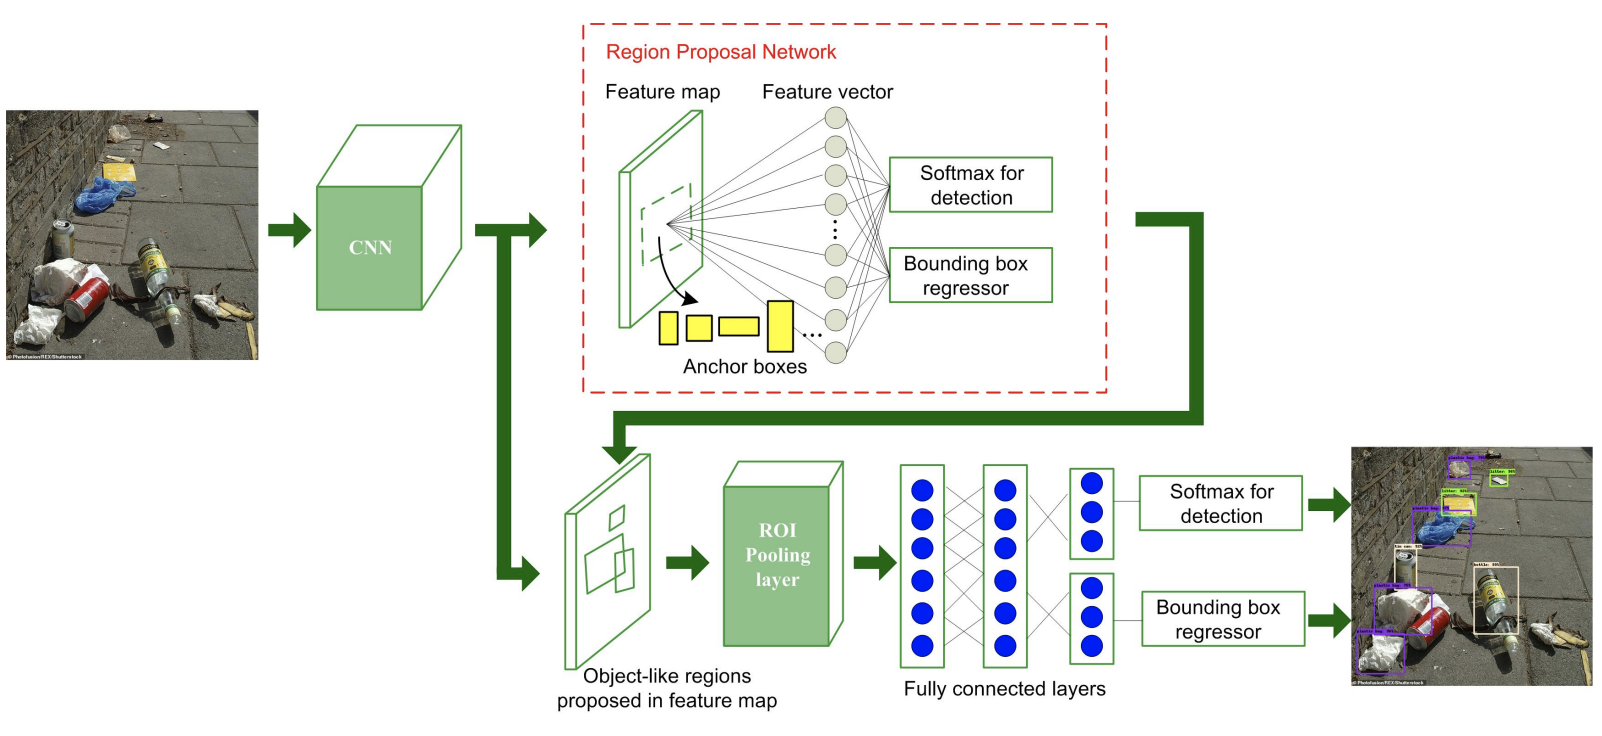
\includegraphics[scale=0.5]{images/faster-rcnn-architecture.png}
    \caption{The architecture of Faster R-CNN\cite{smart-street}.}
    \label{fig:faster-rcnn-architecture}
\end{figure}

Figure \ref{fig:faster-rcnn-architecture} illustrates how Faster R-CNN uses layers known as Region Proposal Networks (RPN) to generate feature maps which are turned into object region proposals. The proposals are projected onto the feature map and objects are detected by classifying the proposals. Now a one-stage detector with a single network, Faster R-CNN, like YOLO\cite{yolov1}, can be trained end-to-end and optimised for detection performance.

\subsection{Litter}

Despite the availability of large data sets such as COCO\cite{lin2015microsoft}, litter is underrepresented due to its geographic and material variation. The Trash Annotations In Context (TACO) initiative aims to tackle this problem with the goal of improving autonomous litter monitoring systems\cite{DBLP:journals/corr/abs-2003-06975}. In its paper, the TACO researchers describe how it can often often be impossible to distinguish between different types of litter due to the small size of the objects and the resolution of the images. Cigarettes, one of the most commonly littered objects, mostly covered an area less than 64x64 pixels in size. This issue compounds with the lack of available data, which they attempt to address using augmentation and transplantation techniques. A Mask R-CNN model was trained, but the lack of annotated images and difficulty detecting small objects significantly impacted the resulting AP performance.

A Clean Europe Network summit meeting\footnote{https://cleaneuropenetwork.eu/en/measuring-litter/aus} concluded that a lack of data is contributing to the difficulty in addressing the environmental issues caused by urban littering. Cities throughout the world are assessing urban cleanliness by means of human audit. Without a practical approach to measuring an index of cleanliness, it will be challenging to properly manage the problem. 

Researchers in Spain proposed a cleanliness index for the city of Granada\cite{sevilla}. As part of its definition litter was weighted based on its classification, with larger objects assigned higher weights. The study used data that was manually collected by humans and provided by the organisation responsible for cleaning the city.

Attempts to quantify litter using automated object detection have been made\cite{cvstreets}. However, the lack of available data forced the researchers to manually collect and annotate images. A camera was attached to a vehicle and placed at a height of two to three meters from the ground. This limited the litter detection to objects within the immediate vicinity of the vehicle. In the paper, it is highlighted that no prior work has been undertaken to develop such an automated approach.

Efforts have also been made to automate the data collection process. Researchers in India have used the Bing Image Search API\footnote{https://www.microsoft.com/cognitive-services/en-us/bing-image-search-api} to gather a large and diverse set of 2561 images that could be used to train a CNN for detecting litter\cite{Mittal2016SpotGarbageSA}. They provide an Android mobile application that can be used by citizens to report litter in their communities. The approach focused on segmenting areas of an images taken by mobile phones, rather than the quantification of litter itself. In their paper, the authors describe how they utilised a pre-trained AlexNet\cite{NIPS2012_c399862d} model to obtain a 90.06\% specificity and 83.96\% sensitivity.

\section{Regression}

The inference of count data involves estimating the unknown parameters of a given probability distribution. The distribution models the number of occurrences of an event, such as train accidents in a given year, or a rate, such as the quantity of litter in a given area.

\subsection{Poisson}

The benchmark parametric model for count data is the Poisson distribution\cite{cameron_trivedi_2013}. Shown in equation \ref{eq:poisson-model}, the model assumes that the response $Y$ follows the Poisson distribution and it is concerned with modelling the effects of explanatory variables on the response through the rate parameter $\mu$. 

\begin{equation}
    E(Y_i) = \mu_i = n_i\theta_i = n_ie^{x_i^t\beta},\hspace{1em}Y_i = Poi(\mu_i)
    \label{eq:poisson-model}
\end{equation}

The unknown rate parameter $\mu$ is defined in terms of units of exposure, which is the length of time during which the events are recorded\cite{cameron_trivedi_2013}. Dependence on the explanatory variables is given by $\theta_i = n_ie^{x_i^t\beta}$ in which the $i$th covariate pattern is explained for exposure $n_i$.

The corresponding link function with offset $\log{n_i}$ is given by:

\begin{equation}
    \log{\mu_i} = \log{n_i} + x_i^t\beta
\end{equation}

The mean and variance of $Y \sim Poi(\mu)$ are both $\mu$ and the probability mass function for the distribution is given in equation \ref{eq:possion-pmf}. 

\begin{equation}
f(y) = \frac{\mu^ye^{-\mu}}{y!},\hspace{1em}y = 0, 1, 2,...
\label{eq:possion-pmf}
\end{equation}

This equality is known as the \textit{equidispersion} property of the Poisson and it is frequently not the case for real-world data. \textit{Overdispersion} is said to occur if the mean exceeds the variance. Similarly, \textit{underdispersion} presents itself if the variance is less than the mean. When data exhibit this property, it needs to be accounted for so that statistical inferences are valid\cite{understanding-poisson}.

Poisson regression models have been applied in many domains including health, finance and manufacturing. In 1992, the number of defects per area in a manufacturing process at the AT\&T Bell Laboratories was studied\cite{defects}. The researchers used the zero-inflated variant of the model to identify the set of conditions under which the mean number of defects was lowest.

\subsection{Negative Binomial}

Violations of the equidispersion property of the Poisson regression model can be dealt with by assuming a negative binomial distribution for the response $Y$, which allows for variances that are not equal to the mean.

The model form is the same as the Poisson and it introduces a new unknown variable $\alpha$ with density:

\begin{equation}
    f(y|\mu,\alpha) = \frac{\Gamma(y + \alpha^{-1})}{\Gamma(y+1)\Gamma(\alpha^{-1})}(\frac{\alpha^{-1}}{\alpha^{-1} + \mu})^{\alpha^{-1}}(\frac{\mu}{\alpha^{-1} + \mu})^y,\hspace{1em}\alpha\ge 0, y=0,1,2,...
\end{equation}

Both $\mu$ and $\alpha$ are estimated during model fitting. It has been suggested that $\alpha$ should be chosen such that the Pearson or deviance static is equal to $n - k$\cite{cameron_trivedi_2013}.

The model reduces to the Poisson if $\alpha = 0$ as it is used to explain the variance which is $Var(Y_i) = \mu_i + \alpha\mu_i^2$ for the NB2 model: the most common implementation of the negative binomial\cite{cameron_trivedi_2013}. This formulation is popular because it allows the modelling of Poisson heterogeneity using a gamma distribution\cite{ncss-neg-bin}.

% Data ========================================================================
% Data summary
% Data collection
% Ethical considerations

\chapter{Data} \label{chapter:data}

The data for the study was collected from three independent sources.

\section{Scottish Index of Multiple Deprivation}

The Scottish Index of Multiple Deprivation (SIMD) is a tool for identifying the places in Scotland where people are experiencing disadvantage across different aspects of their lives \cite{simd}. Published by the Scottish Government, it provides a relative measure of deprivation across many small areas of the country.

The data are a collection of 6,976 data zones which represent areas with roughly equal populations of 700 -- 800 people (Figure \ref{fig:dz-total-populations}.) Each data zone has over 30 deprivation indicators such as crime rate, unemployment rate, and pupil attainment. By combining these indicators into a single index, the data zones are ranked relative to one another, from 1 -- 6,976, where rank 1 is the most deprived area in the country. In total, seven aspects of deprivation are combined: Income, Employment, Health, Education, skills and training, Geographic access to services, Crime, and Housing.

\begin{figure}[h]
    \centering
    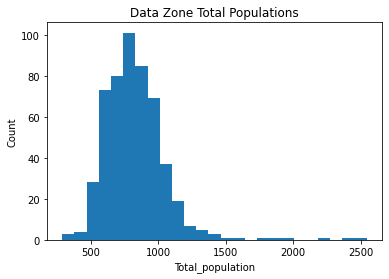
\includegraphics[scale=0.75]{images/dz-total-population.png}
    \caption{The total populations of Glasgow City's 746 data zones.}
    \label{fig:dz-total-populations}
\end{figure}

For the purposes of the study, the subset of data zones located in the Glasgow City council area was obtained, resulting in a collection of 746 data zones with associated deprivation indicators described in \ref{table:simd-deprivation-indicators}. Figure \ref{fig:glasgow-uni-dz} is one such data zone.

A revised version of the January 2020 publication was used for the study, in which the income domain and overall rankings were updated as a result of an error in the original data provided by the Department for Work and Pensions\footnote{https://www.gov.scot/publications/scottish-index-of-multiple-deprivation-2020v2-revision-notice}.

\begin{figure}[h]
    \centering
    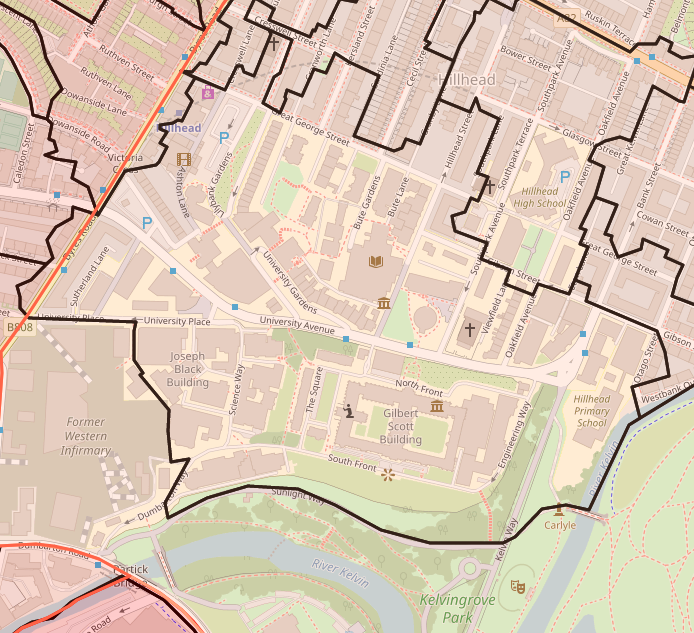
\includegraphics[scale=0.5]{images/glasgow-uni-ward.PNG}
    \caption{The data zone containing the University of Glasgow (S01010379).}
    \label{fig:glasgow-uni-dz}
\end{figure}

\subsection*{Missing Data}

A total of 137 missing indicator values were discovered in the data for Glasgow City. Indicated by a '*' character, the missing value is used when a value cannot be determined, or if the value has been suppressed for disclosure control where small numbers are involved.

To maintain as much information as possible in the small data set, missing values were imputed as the mean of the observed values.

\subsection*{Litter Response}

In order to answer the questions of interest, the amount of litter in each Glasgow City data zone was quantified and added to the SIMD data set as integer counts. The object detection methods used to achieve the creation of this response variable are  described in chapter \ref{chapter:methods}.



\begin{table}[ht!]
    \centering
    \begin{tabular}{||l p{100mm}||} 
     \hline
     \textbf{Indicator} & \textbf{Description} \\ [0.5ex] 
     \hline\hline
     Data\_Zone & Data zone name (string) \\
     Intermediate\_Zone & Intermediate zone name (string) \\
     Council\_area & Council area name (string)  \\
     Total\_population & Area population estimate (integer) \\
     Working\_age\_population & Area working age population estimate using state pension age (integer) \\
     income\_rate & Percentage of people who are income deprived \\
     employment\_rate & Percentage of people who are employment deprived \\
     employment\_count & Number of people who are employment deprived (integer) \\
     CIF & Comparative illness factor (standardised ratio\footnotemark) \\
     ALCOHOL & Hospital stays related to alcohol use (standardised ratio) \\
     DRUG & Hospital stays related to drug use (standardised ratio) \\
     SMR & standardised mortality ratio (standardised ratio) \\
     DEPRESS & Percentage of population being prescribed drugs for anxiety, depression or psychosis \\
     LBWT & Percentage of live singleton births of low birth weight \\
     EMERG & Emergency stays in hospital (standardised ratio) \\
     Attendance & Percentage of school pupil attendance \\
     Attainment & Attainment score of school leavers (float) \\
     no\_qualifications & Working age of people with no qualifications (standardised ratio) \\
     not\_participating & Percentage of people aged 16 -- 19 not participating in education, employment or training \\
     University & Percentage of 17 -- 21 year olds entering university \\
     drive\_petrol & Average drive time to a petrol station in minutes (float) \\
     drive\_GP & Average drive time to a GP surgery in minutes (float) \\
     drive\_PO & Average drive time to a post office in minutes (float) \\
     drive\_primary & Average drive time to a primary school in minutes (float) \\
     drive\_retail & Average drive time to a retail centre in minutes (float) \\
     drive\_secondary & Average drive time to a secondary school in minutes (float) \\
     PT\_GP & Public transport travel time to a GP surgery in minutes (float) \\
     PT\_Post & Public transport travel time to a post office in minutes (float) \\
     PT\_retail & Public transport travel time to a retail centre in minutes (float) \\
     broadband & Percentage of premises without access to super fast broadband (float) \\
     crime\_count & Number of recorded crimes of violence, sexual offences, domestic housebreaking, vandalism, \newline drugs offences, and common assault (integer) \\
     crime\_rate & Number of recorded crimes of violence, sexual offences, domestic housebreaking, vandalism, \newline drugs offences, and common assault per 10,000 people (integer) \\
     overcrowded\_count & Number of people in households that are overcrowded (integer) \\
     nocentralheat\_count & Number of people in households without central heating (integer) \\
     overcrowded\_rate & Percentage of people in households that are overcrowded \\
     nocentralheat\_rate & Percentage of people in households without central heating \\ [1ex] 
     \hline
    \end{tabular}
    \hspace{100mm}
    \caption{Description of the SIMD data zone deprivation indicators.}
    \label{table:simd-deprivation-indicators}
\end{table}

\footnotetext{A value of 100 is the Scotland average for a population with the same age and sex profile.}

\section{Google Street View Images}

To achieve a quantification of litter using object detection, thousands of images depicting the streets of Glasgow City were downloaded from the Google Maps Platform to be used as input to the object detection models. 

Software\footnote{https://github.com/Garee/glasgow-litter} was developed to obtain the images using the Street View Static API\footnote{https://developers.google.com/maps/documentation/streetview/overview}. A random sample of 50 unique locations were generated within each data zone boundary and an image was downloaded at each.

A total of 37,300 images (50 for each data zone) were retrieved at the maximum resolution of 640x640 pixels at a pitch of 0 degrees with a 90 degree field of view from the source camera on the vehicle. Figure \ref{fig:street-view-image} is one such example.

\begin{figure}[h]
    \centering
    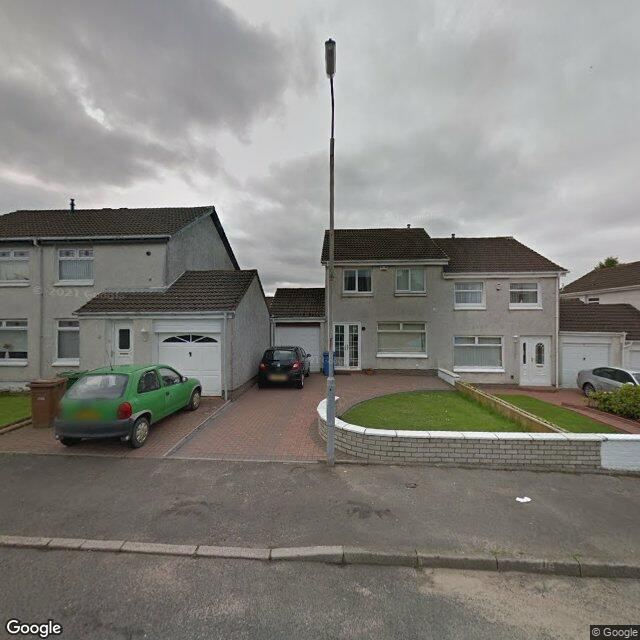
\includegraphics[scale=0.5]{images/street-view-image.jpg}
    \caption{A typical image of a Glasgow City street retrieved using the Google Maps Platform.}
    \label{fig:street-view-image}
\end{figure}

\subsection*{Privacy}

The images returned by Google have human faces and vehicle license plates automatically blurred to protect the privacy of individuals.

\section{Public Recycling Facility Locations}

The location and details of Glasgow City's 741 public recycling facilities were requested in JSON format from the public map\footnote{https://glasgowgis.maps.arcgis.com/apps/webappviewer/index.html?id=345f389a91ff4f1fa193b24df832fb05} hosted and maintained by Glasgow City Council.

Software was developed to count the number of facilities within each data zone boundary and add them to the SIMD data set as integers such that the count could be used as a potential explanatory variable.

% Methods =====================================================================
% Data Analysis

\chapter{Methods} \label{chapter:methods}

\section{Litter Detection}

To quantify the amount of litter in a data zone, the computer vision technique of object detection was performed to identify litter in the street view images that were randomly sampled from within that data zone. This technique localised any litter in an image and assigned it to the litter target class. To this end, the technique took as input a single street view image and produced zero or more $x_1,y_1,x_2,y_2$ bounding box co-ordinates that determined the location of the litter within that image. This task was repeated fifty times for each data zone before summing the number of bounding boxes to produce an overall count of litter. The location of the litter within the image was not of interest for the objectives of this project.

\subsection{Data Preparation}

\paragraph{Data Labelling}

I personally hand annotated 7,260 street view images of Glasgow City to produce a collection of labelled images that could be used to train the object detection models. Only a subset of 1,219 images contained litter. The open source data labelling tool Label Studio\footnote{https://labelstud.io} was used for this process.

As litter are generally small objects, and the images were limited to a resolution of 640x640 pixels, it was often impossible to determine the type of litter that was being annotated. For this reason only a single target class of "litter" was used. Fortunately, this was enough for the goal of quantification. It also avoids the issue of an imbalance label distribution, in which some classes are significantly more frequent than others.

To maximise the performance of the resulting models it was important to annotate consistently and with consideration. As I was the only individual labelling, I did not have to worry about the potential variability introduced by the subjectivity of multiple participants. A tight box was annotated around the litter, and deposits of multiple litter objects were annotated individually.

\paragraph{Data Split}

The images were split into training, validation and test data sets using an allocation of 70\%, 20\%, and 10\% respectively. The motivation was to prevent model over-fitting in which it hyper-specifies to the training data, and does not generalise well to never before seen images. When this occurs, the loss function that determines how close the model is to making an accurate prediction ever decreases for the training data set, but eventually increases for the held-out validation data set.

As the validation data set was used heavily during model creation and influenced the chosen model, a separate independent test data set was also held back. This was used to produce evaluation metrics at the end of the project, to gauge a sense of how well the final model performs.

In order to avoid train-test bleed in which the test data set is overly similar to the training data set, verification was performed to ensure that there were no duplicate images.

\paragraph{Data Preprocessing}

Preprocessing steps were applied to all three data set splits in order to standardise them. Resizing was not necessary as all images were collected at a resolution of 640x640 pixels. 

In order to train our model to know that a street view may exist without litter, which is often the case, it was important to include null labelled images in the training data set. This is an important step to reduce false positives. To achieve this, a null filter was applied that guaranteed that at least 80\% of the training data contained labels, while still allowing for those with none.

A contrast preprocessing step was applied to exaggerate the differences between neighbouring pixels in order to improve edge detection. This is helpful as google street view images are not all alike; they are taken at different times of day and in different weather conditions. By adjusting the contrast using adaptive equalisation to smooth the contrast, the resulting model may be more accurate.

\paragraph{Data Augmentation}

Image augmentations were applied to increase the size of the training set. These made slight alterations to the collected training data in order to produce new images, and therefore more information, for the model to learn from. This was an efficient way to generate thousands more training images without having to perform additional time consuming manual labelling. The ground truth images were not augmented, as these were used during evaluation procedures.

The mosaic augmentation combined four source images into one by simulating four random crops while maintaining the relative scale of the litter. It aims to improve performance in terms of translation, and it also varies the amount of litter present in the images. This is because a mosaic image can potentially include litter from multiple other image sources. This was an important augmentation as it greatly increased the number of available training images.

Table \ref{table:model-augmentations} summarises the models that were produced using different combinations of data preprocessing and augmentation techniques.

\begin{table}[ht!]
    \centering
    \begin{tabular}{|l| |c|} 
     \hline
      \textbf{Augmentations} & \textbf{\# Training Images} \\
     \hline\hline
     None & 853 \\
     Mosaic x2 & 1,706  \\
     Mosaic x2, Auto-adjust Contrast & 1,706  \\
     Mosaic x3 & 2,559\\
     Mosaic x3, 5\% Noise & 2,559 \\
     Mosaic x3, Auto-adjust Contrast, 5\% Noise & 2,559 \\
     \hline
    \end{tabular}
    \hspace{100mm}
    \caption{The data augmentations used for each trained model.}
    \label{table:model-augmentations}
\end{table}

\subsection{Hardware}

All object detection models were created using a personal computer to minimise compute costs. The time taken to train a single object detection model on the training data was typically in the region of 2 -- 5 hours, depending on the chosen number of epochs. Table \ref{table:hardware} describes the key component specifications.

\begin{table}[ht!]
    \centering
    \begin{tabular}{|c| |c|} 
     \hline
     \textbf{Component} & \textbf{Description} \\ [0.5ex] 
     \hline\hline
     CPU & AMD Ryzen 5 5600X \\
     GPU & NVIDIA RTX 3060 12GB \\
     RAM & 32GB 3200Mhz Dual Channel  \\
     \hline
    \end{tabular}
    \hspace{100mm}
    \caption{The key hardware specifications used during model creation.}
    \label{table:hardware}
\end{table}

\subsection{Yolov5}

Multiple Yolov5 object detection models were trained and evaluated. This involved iteratively, in batches, improving the way the models mapped images to predictions. Techniques such as transfer learning, hyper-parameter tuning, and the aforementioned data augmentations were performed in an attempt to produce the best training results possible.

\paragraph{Transfer Learning}

To start from a strong foundation, the transfer learning method was used to obtain application knowledge from an existing model and reuse it as the basis for the new task of detecting litter. Learning was transferred from the YOLOv5s model which had been pre-trained on the COCO data set\footnote{https://cocodataset.org}. This data set contains 80 classes, a few of which are potentially litter e.g., bottle, knife and fork. Transfer learning is expected to produce better results than starting from scratch as the weights have already been optimised for a related task. The YOLOv5s model was selected as it requires less memory to train, and is faster to run than alternatives such as YOLOv5x\footnote{https://github.com/ultralytics/yolov5\#pretrained-checkpoints}. The resource intensive alternatives would likely be more accurate, but it was important that the model complement the hardware at hand.

\paragraph{Batch Size} 

As it is not possible to provide the entire training data set to the model at once, it must be split up and provided in batches. The largest batch size that the hardware allowed for was used to decrease training times. This was 32 with a GPU memory pool of 12GB.

\paragraph{Epochs} 

An epoch occurs when the entirety of the training data has been passed through the model's neural network once. The choice of number of epochs is an important one as it greatly influences whether over or under-fitting occurs due to the iterative nature of the optimisations that occur during training. Too many epochs and the model will over fit. Too few, and the model is not given iterations to successfully optimise to the data. Figure \ref{fig:epochs} shows why 450 epochs was the chosen amount. This is the point at which the validation object loss starts decreasing, while the training loss continues to decrease. This is the tell tale sign that over fitting is starting to occur.

\begin{figure}[h]
    \centering
    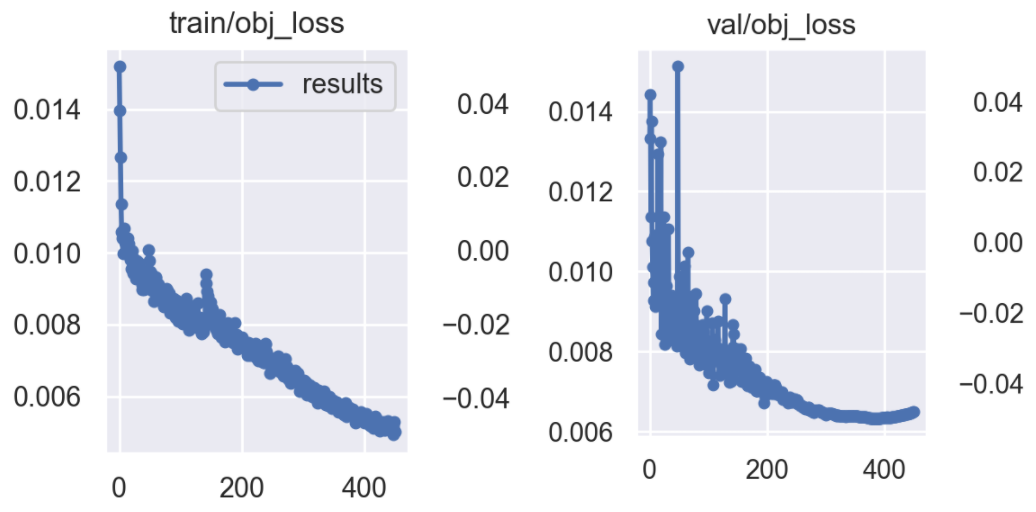
\includegraphics[scale=0.5]{images/train-val-obj-loss.png}
    \caption{The object loss for training and validation data sets over 450 epochs.}
    \label{fig:epochs}
\end{figure}

\paragraph{Iterations} 

With a batch size of 32 and 2,559 training images, it would take $\ceil{2,559 / 32} = 80$ iterations for a single epoch.

\paragraph{Hyperparameter Tuning}

Hyperparameter tuning was performed in an attempt to choose the optimal set of parameters for the model. The Yolov5 project offers a method of hyperparameter evolution that uses a genetic algorithm for optimisation. This process was run using the best performing model as a base scenario from which to evolve from. The value to maximise, \textit{fitness}, was defined as a weighted combination of metrics: mAP@0.5 contributes 10\% of the weight and mAP@0.5:0.95 contributes the remaining 90\%. The genetic algorithm had a 90\% probability and a 0.04 variance to create new offspring based on a combination of the best parents from all previous generations. Due to how expensive this evolution process is, only 10 generations were completed which limits its effectiveness.

\subsection{Faster RCNN}

In addition to Yolo-based models, Faster RCNN models were trained and evaluated for comparison using detectron2\footnote{https://github.com/facebookresearch/detectron2}. These models were created using the same augmented data and training settings described in previous sections. However, there was no built-in method for automated hyperparameter tuning. Fortunately, as described in the chapter \ref{chapter:results}, this would not be necessary as the Yolo-based models were the better performers.

\subsection{Model Selection}

The standard evaluation metric to use for model selection is the mean average precision, which quantifies the performance of an object detector across all validation images and at different confidence thresholds. Table \ref{table:model-mAP} lists the \textit{mAP} scores for a select highlight of trained models.

\begin{table}[ht!]
    \centering
    \begin{tabular}{|l| |l|} 
     \hline
     \textbf{Model} & \textbf{mAP} \\
     \hline\hline
     Yolov5s with No Augmentations & 38.67 \\
     Yolov5s with Mosaic x2 & 40.60  \\
     Yolov5s with Mosaic x2, Auto-adjust Contrast & 40.12  \\
     Yolov5s with Mosaic x3 & 52.65 \\
     Yolov5s with Mosaic x3, 5\% Noise & 43.16 \\
     Yolov5s with Mosaic x3, 5\% Noise and Tuned & 58.19 \\
     Yolov5s with Mosaic x3, Auto-adjust Contrast, 5\% Noise & 42.21 \\
     Faster RCNN with No Augmentations & 26.50 \\
     Faster RCNN with Mosaic x3 & 55.12 \\
     \hline
    \end{tabular}
    \hspace{100mm}
    \caption{The mean average precision results for a subset of the trained object detection model.}
    \label{table:model-mAP}
\end{table}

The hyperparameter tuned Yolov5s model trained on mosaic and noise augmented data produced the best result with an mAP of 58.19. Figures \ref{fig:pr-curve} and \ref{fig:f1-curve} show the associated precision-recall and F1 curves, which also happened to be the best. 

\begin{figure}[h]
    \centering
    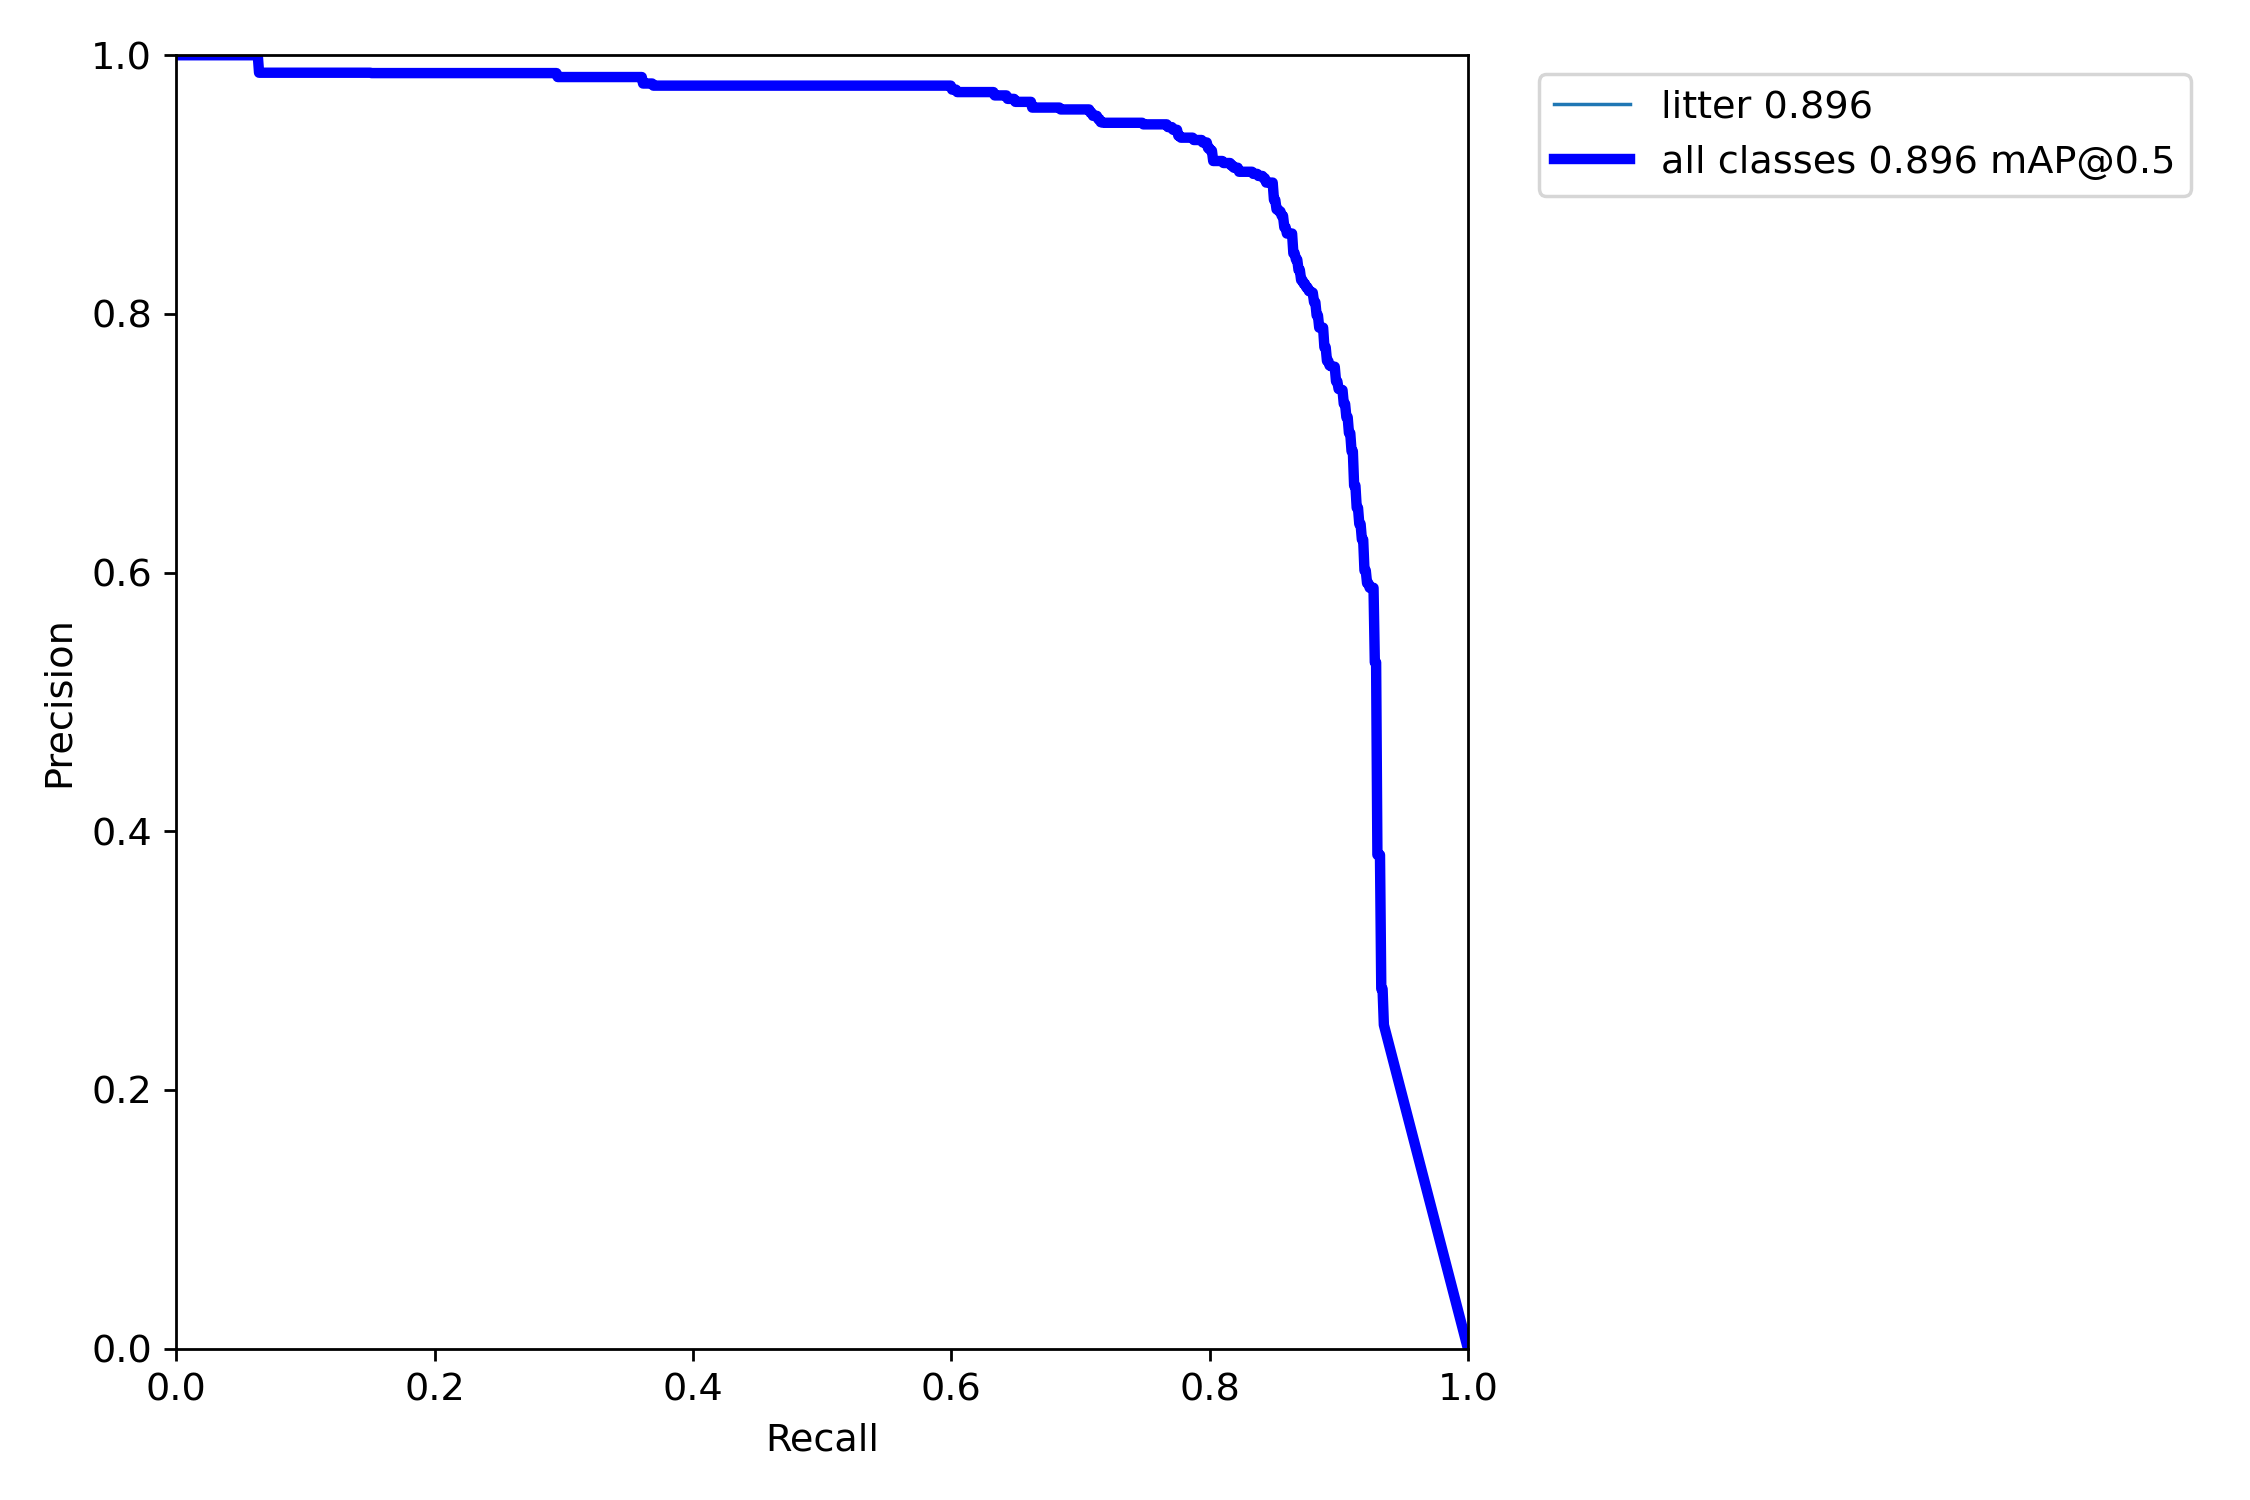
\includegraphics[scale=0.5]{images/pr-curve.png}
    \caption{The precision-recall curve of the chosen model applied to the validation data.}
    \label{fig:pr-curve}
\end{figure}

\begin{figure}[h]
    \centering
    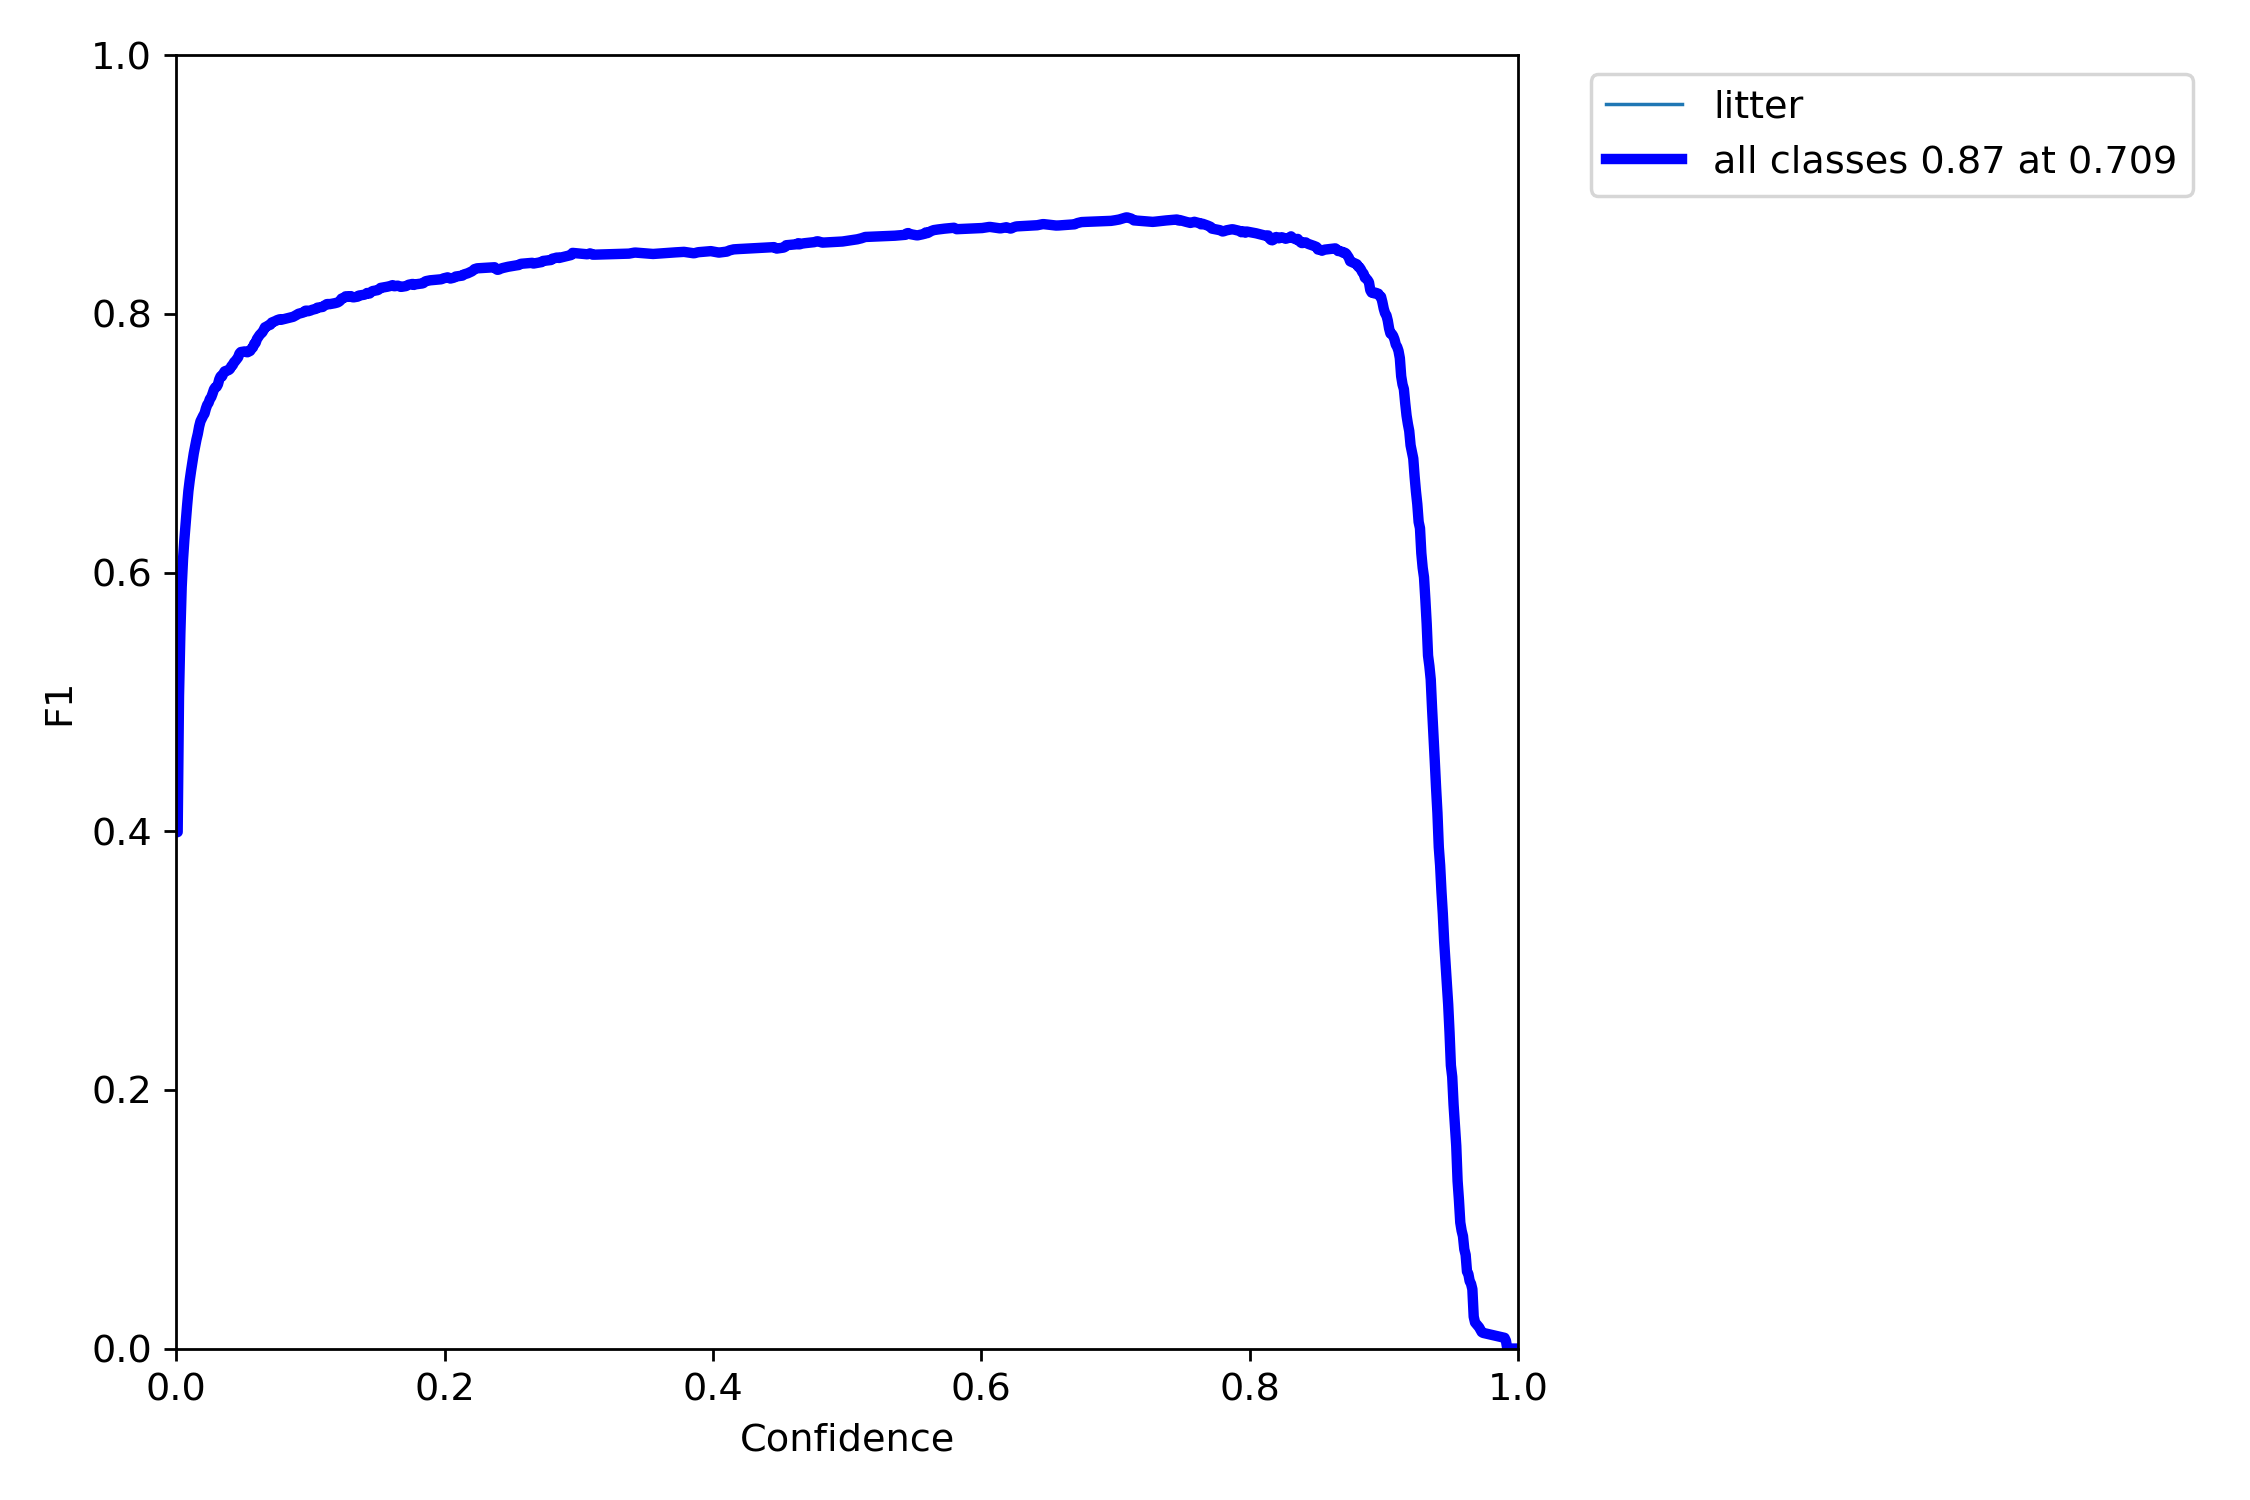
\includegraphics[scale=0.5]{images/f1-curve.png}
    \caption{The F1 curve of the chosen model applied to the validation data.}
    \label{fig:f1-curve}
\end{figure}

Figure \ref{fig:confusion-matrix-validation} shows the associated confusion matrix. The model performed with a 89\% true positive rate, and an 11\% false positive rate on the validation data set. This means that 9 of every 10 occurrences of litter were correctly identified as litter.

For these reasons it was the model chosen from which to perform the litter quantification of each data zone of Glasgow City.

\begin{figure}[h]
    \centering
    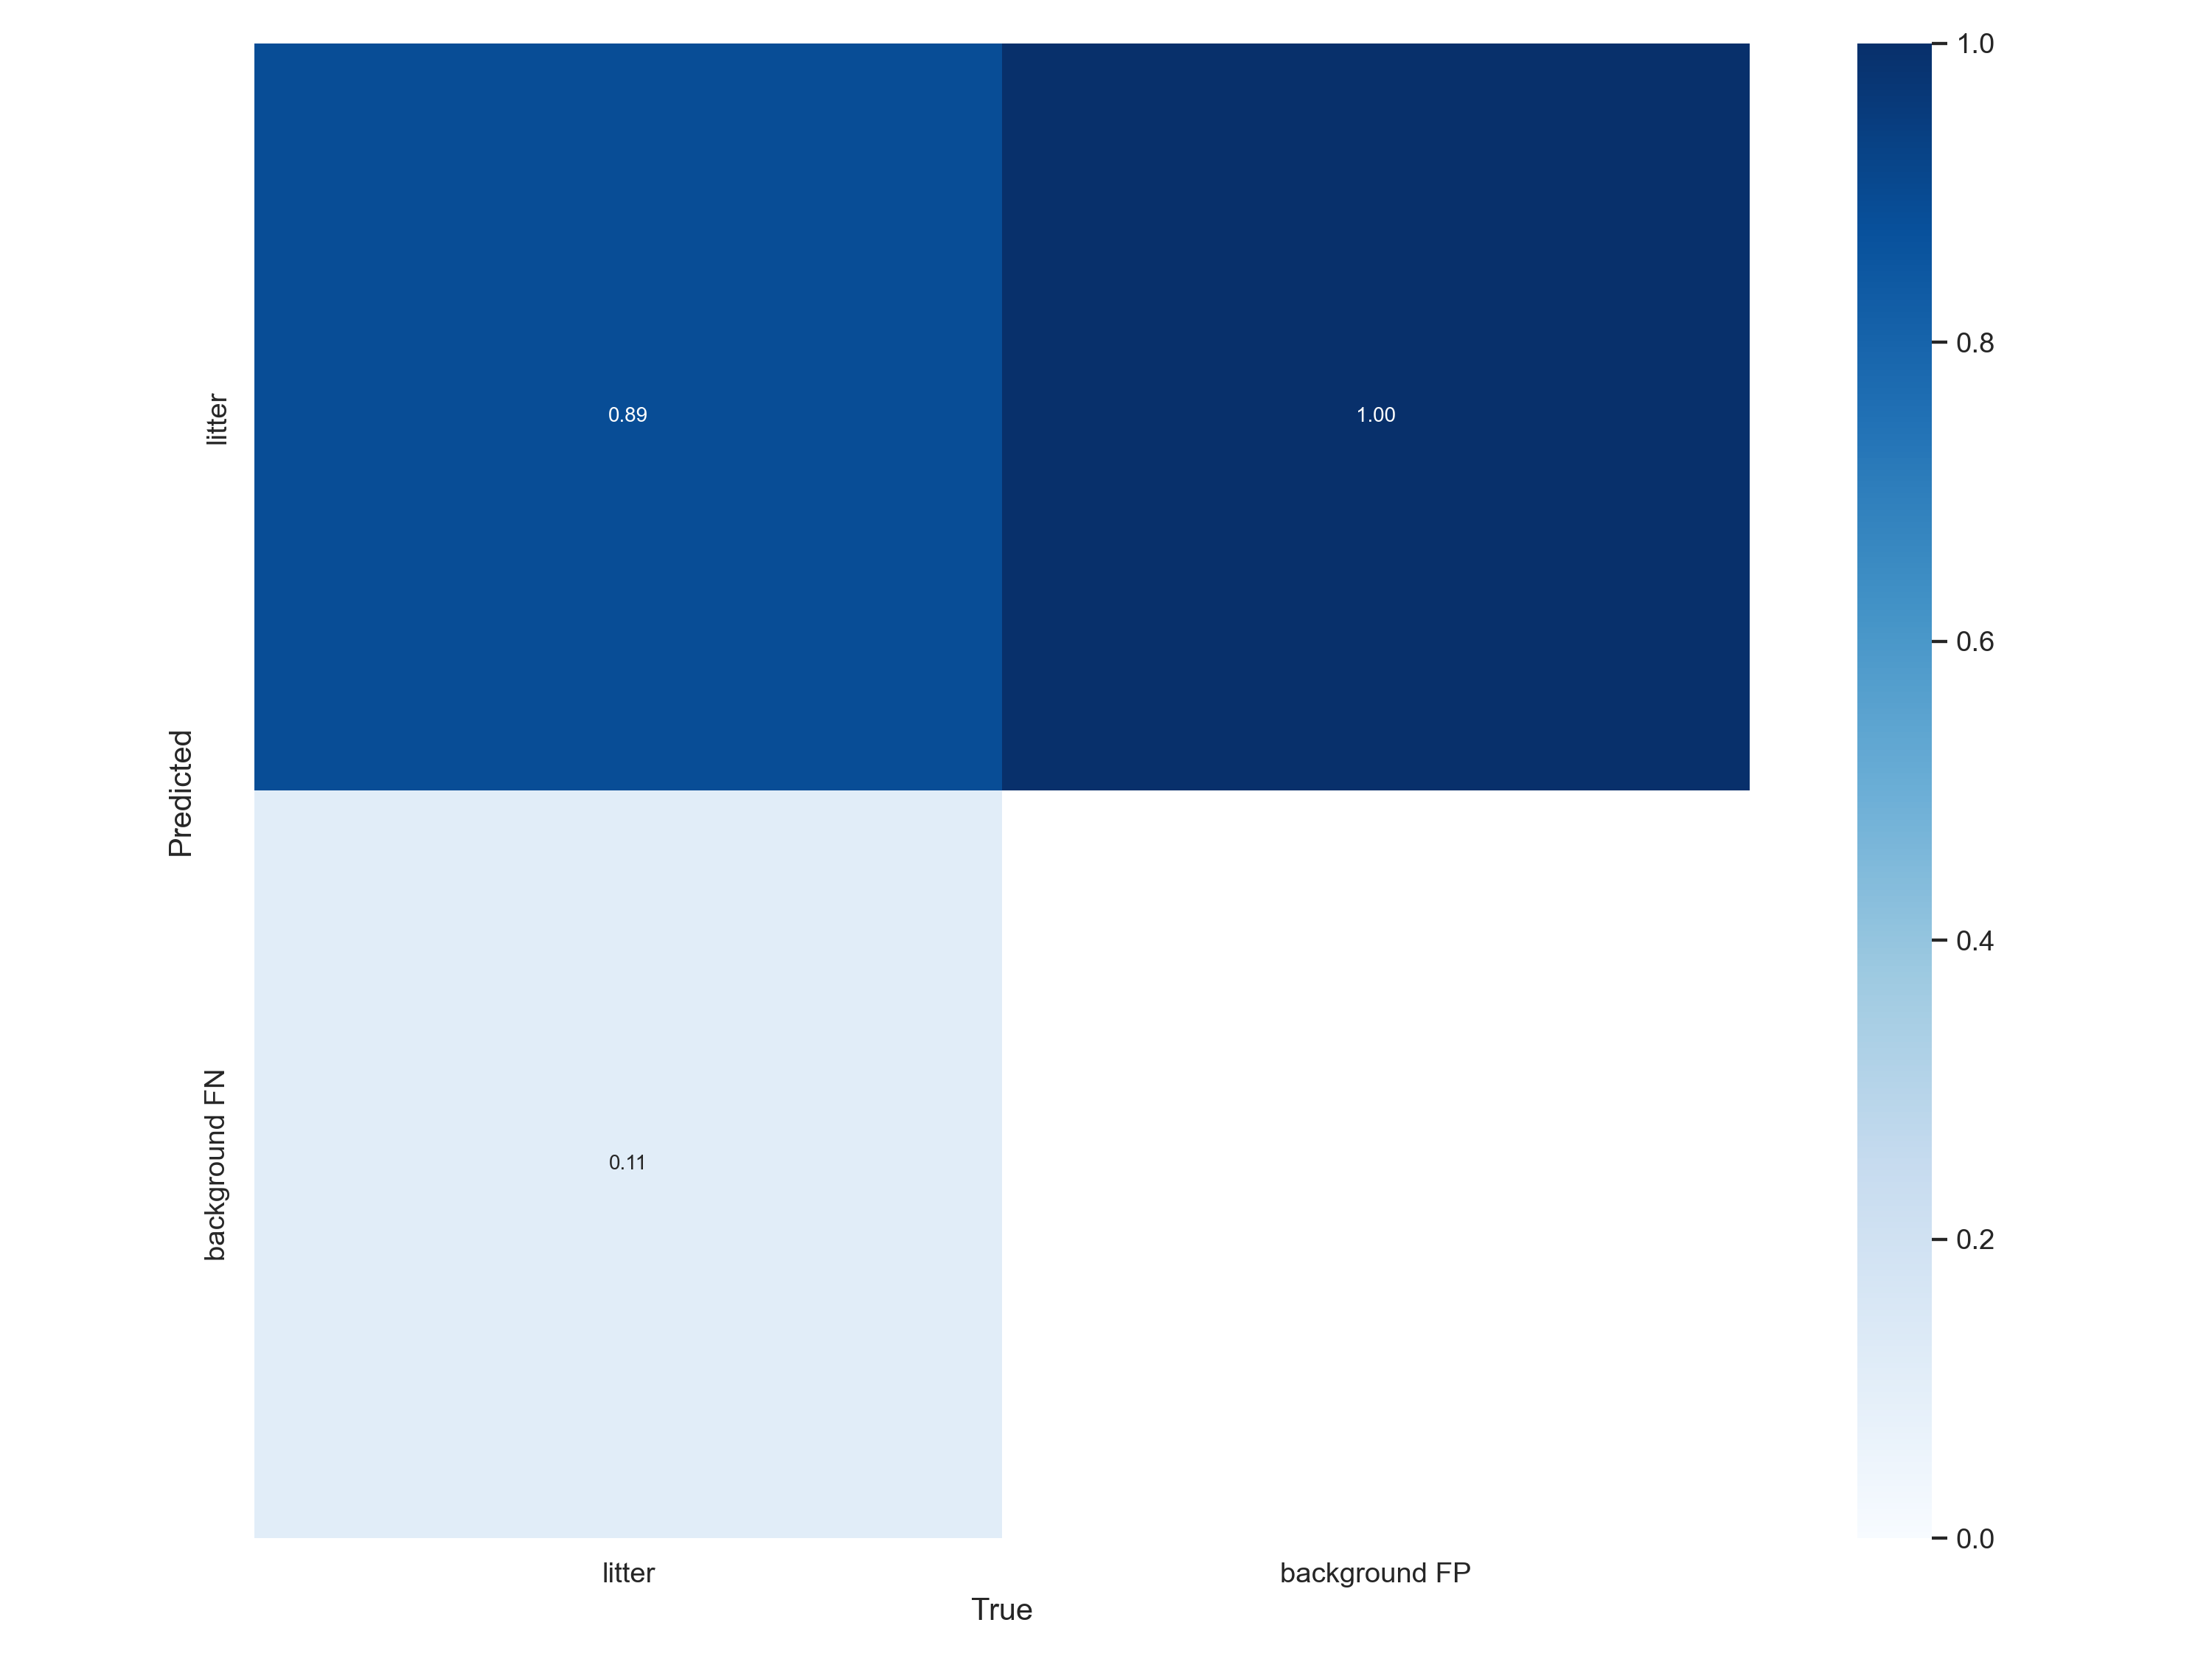
\includegraphics[scale=0.45]{images/final-model-confusion-matrix-val.png}
    \caption{The confusion matrix of chosen model on the validation data.}
    \label{fig:confusion-matrix-validation}
\end{figure}

\subsection{Model Inference}

Figure \ref{fig:litter-histogram} shows the number of litter objects detected within fifty randomly sampled images for each data zone. The count ranges from 0 -- 58 objects and the average number of littered objects was per data zone was 10. Software was developed to add these counts to the SIMD data set as a response variable in preparation for regression.

\begin{figure}[h!]
    \centering
    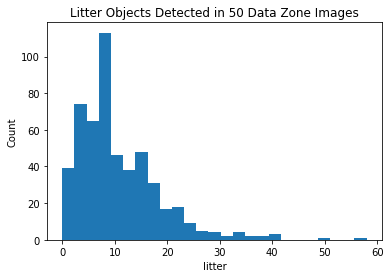
\includegraphics[scale=0.75]{images/litter-hist.png}
    \caption{The number of detected litter objects in each data zone.}
    \label{fig:litter-histogram}
\end{figure}


\section{Regression}

Count data regression was performed on the modified SIMD data set using generalised linear models to answer the question of interest. Is there a relationship between any of Glasgow City's deprivation indicators, and the amount of litter on its streets?

\subsection{Data Preparation}

\paragraph{Standardisation} 

Standardisation was performed as many of the features were not recorded on the same scale. For example, the \textit{crime\_rate} was measured in units of per 10,000 people, whereas the \textit{employment\_rate} is the percentage of people who are income deprived. It is important to re-scale the features to be comparable as the interpretation of regression coefficients is sensitive to the scale of the inputs. The standardisation method applied was Z score which produces a mean of 0 and a standard deviation of 1:

\begin{equation}
    Z = \frac{x - \mu}{\sigma}
\end{equation}

\paragraph{Missing Data} 

As described in chapter \ref{chapter:data}, 137 missing values were imputed using the mean of the observed values from the other observations. It is important to retain as much information as possible to train with as the data set is small.

\subsection{Exploratory Analysis}

\paragraph{Correlations}

Figure \ref{fig:correlation-matrix} shows the features of the data that are most positively and most negatively correlated with the response variable. Pearson's correlation coefficient tells us that as \textit{no\_qualifications}, \textit{income\_rate}, \textit{CIF}, \textit{employment\_rate}, \textit{EMERG}, \textit{DEPRESS}, \textit{SMR}, and \textit{ALOCOHOL} increase, so does the amount of the litter. Similarly, as \textit{Attainment} and \textit{Attendance} increase, the amount of litter decreases. The strength of these correlations are moderate, suggesting that there may be an association and a relationship with litter. For this reason, these features were used as the explanatory variables from which to construct regression models.

The positively correlated features are deprivation indicators that we would strive to keep low. For example, we would like to minimise \textit{no\_qualifications} as it is the ratio of working age people with no qualifications. This tells us that we may see litter increase in areas where qualifications are rarer. The same can be said for the other positively correlated features.

On the other hand, the negatively correlated features are related to deprivation indicators that we would like to see maximised. Namely, the percentage of pupils attending school and the attainment score of those leaving school. This tells us that as these decrease, or in other words get worse, the amount of litter increases.

It should be noted that a change in one of these explanatory variables is not necessarily an explanation for a change in the amount of litter. Correlation is not causation, and it is possible that there is a third yet unidentified causal explanatory variable that both are related to.

\paragraph{Multicollinearity}

Both \textit{income\_count} and \textit{employment\_rate} were also identified as some of the most correlated explanatory variables. However, as they are highly correlated with \textit{income\_rate} and \textit{employment\_rate} they were omitted from further analysis to avoid issues with multicollinearity. This occurs when the independent variables in regression model are related. By definition, to be independent variables they should be independent in nature. If not addresses, the resulting regression coefficients may be unstable.

\begin{figure}[h]
    \centering
    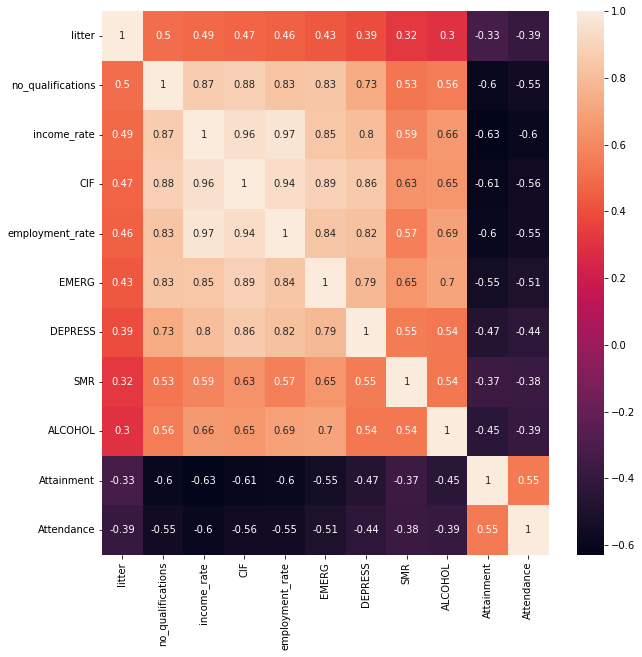
\includegraphics[scale=0.5]{images/corr-matrix.png}
    \caption{The features that were most positively and negatively correlated with litter.}
    \label{fig:correlation-matrix}
\end{figure}


% http://www.stat.columbia.edu/~gelman/research/published/standardizing7.pdf

\subsection{Poisson Regression}

The first model $Y \sim Poi(\mu)$ assumes a Poisson distribution where $\mu$ is defined as the number of litter objects detected in fifty street view images randomly sampled from a data zone in Glasgow City.

Using the ten explanatory variables described during exploratory analysis, forward stepwise feature selection was performed to identify the features which produced the best fit using the Akaike information criterion (AIC) as the selection criteria. With the aim of producing easily interpretable model, the resulting coefficients are outlined in figure \ref{fig:pos-coeff}.

There are statistically significant features such as \textit{income\_rate} where $p < .05$. For example, \textit{Attendance}, \textit{income\_rate}, and \textit{no\_qualifications}. However as the model fit is poor, we cannot conclude that there are any significant relationships.

As the variance in GLMs are not constant, but vary with the mean, we cannot rely on the raw response residuals to assess model fit. The variance is equal to the mean for the Poisson model therefore we use the Pearson chi-squared statistic instead. The Pearson statistic is $\chi^2 = 1940.50$ which is very large when compared to the $\chi^2(511)$ distribution, indicating a poor fit if the Poisson is the correct model for the response.

\begin{figure}[h]
    \centering
\footnotesize
\begin{verbatim}
                     Generalized Linear Model Regression Results                  
==============================================================================
Dep. Variable:                 litter   No. Observations:                  522
Model:                            GLM   Df Residuals:                      511
Model Family:                 Poisson   Df Model:                           10
Link Function:                    Log   Scale:                          1.0000
Method:                          IRLS   Log-Likelihood:                -1953.3
Date:                Mon, 14 Mar 2022   Deviance:                       1845.3
Time:                        20:02:07   Pearson chi2:                 1.94e+03
No. Iterations:                     5   Pseudo R-squ. (CS):             0.8038
Covariance Type:            nonrobust                                         
=====================================================================================
                        coef    std err          z      P>|z|      [0.025      0.975]
-------------------------------------------------------------------------------------
Intercept             2.2891      0.014    158.647      0.000       2.261       2.317
ALCOHOL              -0.0103      0.019     -0.556      0.578      -0.047       0.026
SMR                   0.0348      0.017      2.073      0.038       0.002       0.068
Attainment            0.0146      0.018      0.792      0.428      -0.022       0.051
DEPRESS               0.0451      0.026      1.729      0.084      -0.006       0.096
EMERG                -0.0170      0.031     -0.547      0.585      -0.078       0.044
employment_rate      -0.1600      0.054     -2.951      0.003      -0.266      -0.054
CIF                  -0.0758      0.057     -1.335      0.182      -0.187       0.035
Attendance           -0.0908      0.018     -5.124      0.000      -0.125      -0.056
income_rate           0.3074      0.062      4.938      0.000       0.185       0.429
no_qualifications     0.2338      0.030      7.862      0.000       0.176       0.292
=====================================================================================
\end{verbatim}
\normalsize
    \caption{The coefficients of the Poisson regression model using the training data.}
    \label{fig:pos-coeff}
\end{figure}

\paragraph{Overdispersion}

If the assumption that the variance is equal to the mean does not hold then overdispersion may occur. This is potential explanation for the poor model fit as while the regression parameter estimates are consistent, their standard errors will be incorrect. For this reason, models which do not make this assumption were developed.

\subsection{Negative Binomial Regression}

The next model $Y \sim NegBin(\mu, \alpha)$ introduces a dispersion parameter $\alpha$ and assumes a Negative Binomial distribution for the response which allows for a variance larger than the mean.

Once again, using the ten explanatory variables described during exploratory analysis, forward stepwise feature selection was performed using AIC. The resulting coefficients are outlined in figure \ref{fig:nb-coeff}.

The only coefficients that may be statistically significant, where $p < .05$, are \textit{Attendance}, \textit{income\_rate} and \textit{no\_qualifications}.

The Pearson statistic is $\chi^2 = 369$ which is smaller than the $\chi^2(511)$ distribution, indicating that the model fits if the Negative Binomial is the correct model for the response.

\begin{figure}[h]
    \centering
\footnotesize
\begin{verbatim}
                     Generalized Linear Model Regression Results                  
==============================================================================
Dep. Variable:                 litter   No. Observations:                  522
Model:                            GLM   Df Residuals:                      511
Model Family:        NegativeBinomial   Df Model:                           10
Link Function:                    Log   Scale:                          1.0000
Method:                          IRLS   Log-Likelihood:                -1625.1
Date:                Mon, 14 Mar 2022   Deviance:                       379.20
Time:                        20:03:53   Pearson chi2:                     369.
No. Iterations:                     6   Pseudo R-squ. (CS):             0.2733
Covariance Type:            nonrobust                                         
=====================================================================================
                        coef    std err          z      P>|z|      [0.025      0.975]
-------------------------------------------------------------------------------------
Intercept             2.2866      0.031     73.160      0.000       2.225       2.348
ALCOHOL              -0.0020      0.047     -0.043      0.966      -0.094       0.090
SMR                   0.0387      0.042      0.923      0.356      -0.044       0.121
Attainment           -0.0023      0.042     -0.053      0.957      -0.085       0.081
DEPRESS               0.0260      0.063      0.415      0.678      -0.097       0.149
EMERG                -0.0418      0.078     -0.539      0.590      -0.194       0.110
employment_rate      -0.2006      0.135     -1.484      0.138      -0.466       0.064
CIF                  -0.0674      0.140     -0.481      0.631      -0.342       0.207
Attendance           -0.0903      0.041     -2.208      0.027      -0.170      -0.010
income_rate           0.3367      0.156      2.162      0.031       0.031       0.642
no_qualifications     0.2660      0.071      3.737      0.000       0.126       0.405
=====================================================================================
\end{verbatim}
\normalsize
    \caption{The coefficients of the Negative Binomial regression model using the training data.}
    \label{fig:nb-coeff}
\end{figure}

\paragraph{Bonferroni Correction}

The multiple testing problem describes the fact that as our number of tests for significant effects increase, so does the likelihood of a false positive arising. To mitigate against this, Bonferroni Correction was applied to guard against the bias of repeated testing effects. The coefficient p-values were adjusted such that they are unlikely to be significant through random chance. This divides the significance level $\alpha = .05$ by the number of tests, which has the unfortunate side effect of decreasing the likelihood that a true effect is detected when true.

The resulting p-values all exceeded the new significance level and we therefore conclude that none of the explanatory variables are significant.

\subsection{Model Selection}

The Poisson model did not produce an adequate goodness-of-fit statistic on the training or validation data. However, the Negative Binomial model did, and it is for this reason it was selected as the final model. Figure \ref{fig:predicted-vs-actual-valid} shows that although our Pearson chi-squared statistic suggests a good fit, when applied to the validation data the model does not produce very accurate results.

\begin{figure}[h]
    \centering
    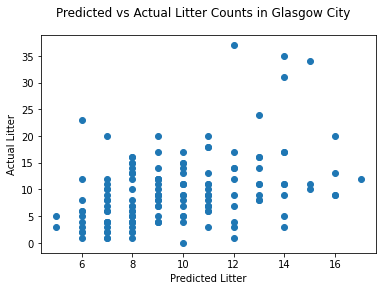
\includegraphics[scale=0.75]{images/valid-predicted-vs-actual-nb.png}
    \caption{The predicted litter counts vs the actual counts for the validation data.}
    \label{fig:predicted-vs-actual-valid}
\end{figure}

% Results =====================================================================
% https://moodle.gla.ac.uk/mod/resource/view.php?id=1517002

\chapter{Results} \label{chapter:results}

\section{Litter Detection}

The confusion matrix in figure \ref{fig:fm-confusion-matrix} illustrates that the model had a 86\% true positive rate, and a 14\% false positive rate, when applied to the test data. We should expected slightly over one in every ten detected litter objects to not actually be litter. This rate is worse than the result produced using the validation data, but not by much.

\begin{figure}[h]
    \centering
    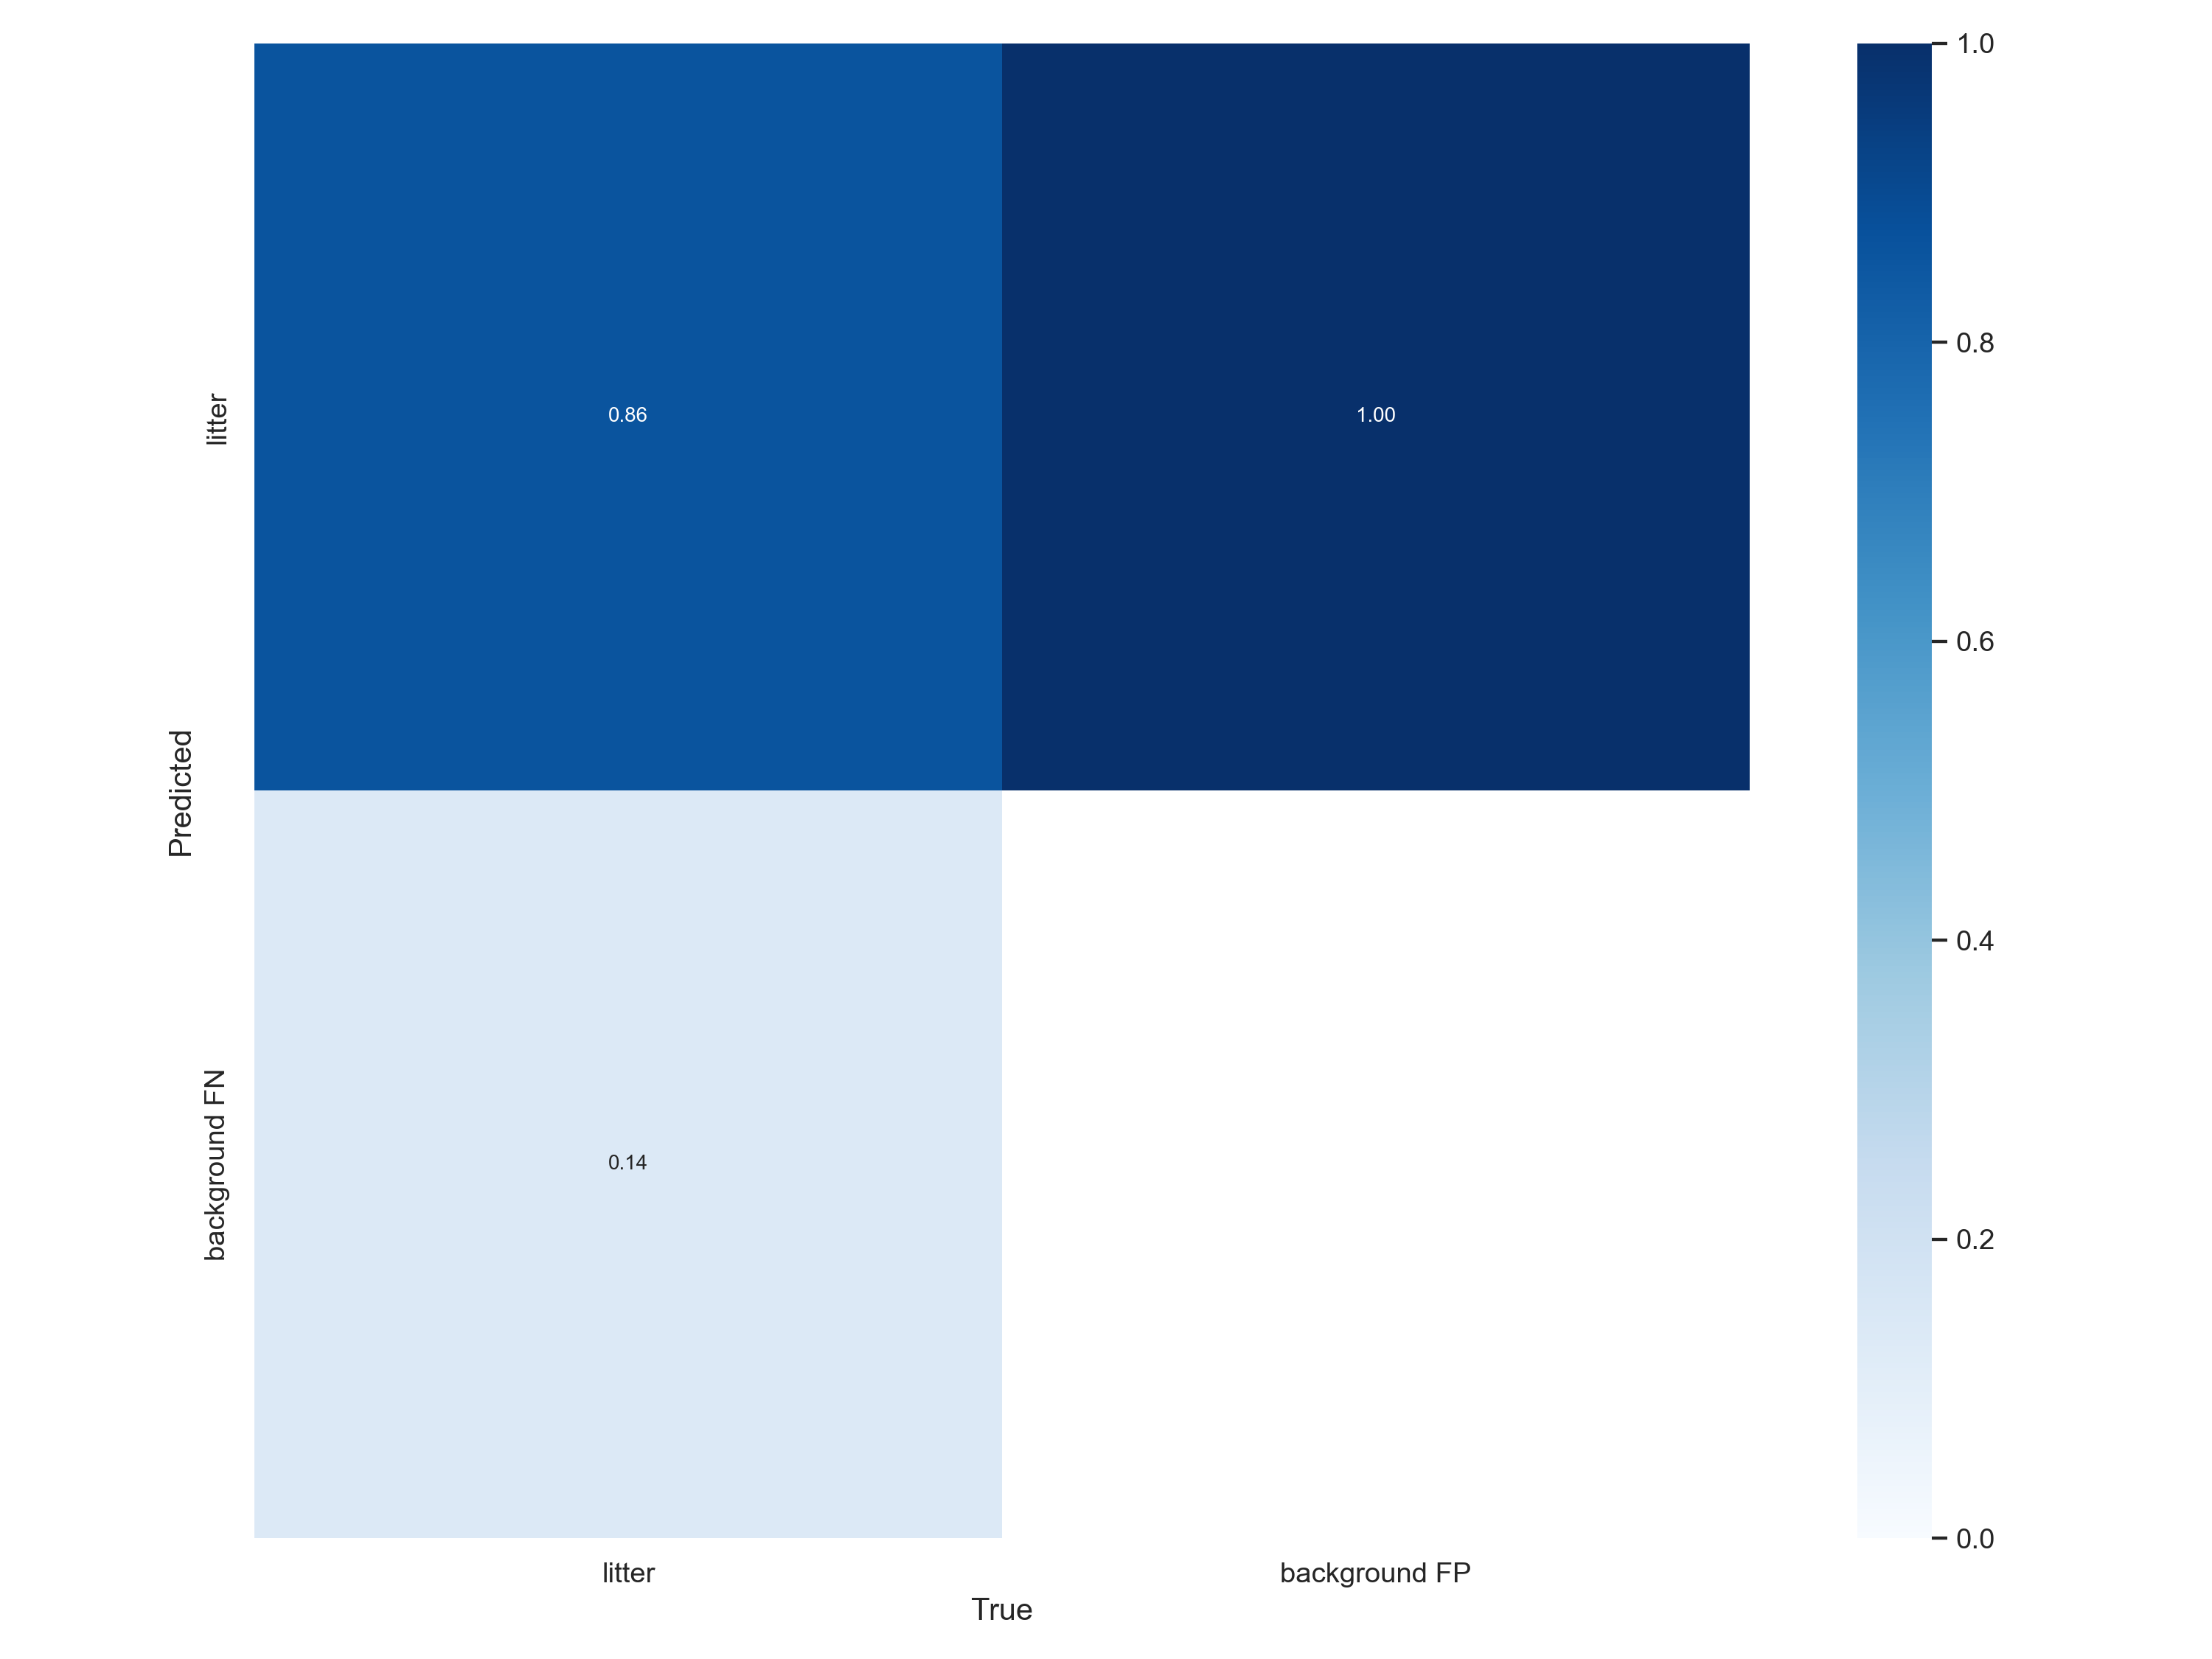
\includegraphics[scale=0.45]{images/fm-confusion-matrix.png}
    \caption{The confusion matrix of the litter detection model when applied to the test data.}
    \label{fig:fm-confusion-matrix}
\end{figure}

Figure \ref{fig:4-in-bush} is a good example of the litter detection model working well. It has successfully identified four small litter objects in the scene, without false positives or false negatives. However, it is certainly not perfect and may detect unexpected objects as litter if they appear similar enough. Figure \ref{fig:sandbag} shows the failings of the model as it detects a white roadside sandbag as litter.

\begin{figure}[h!]
    \centering
    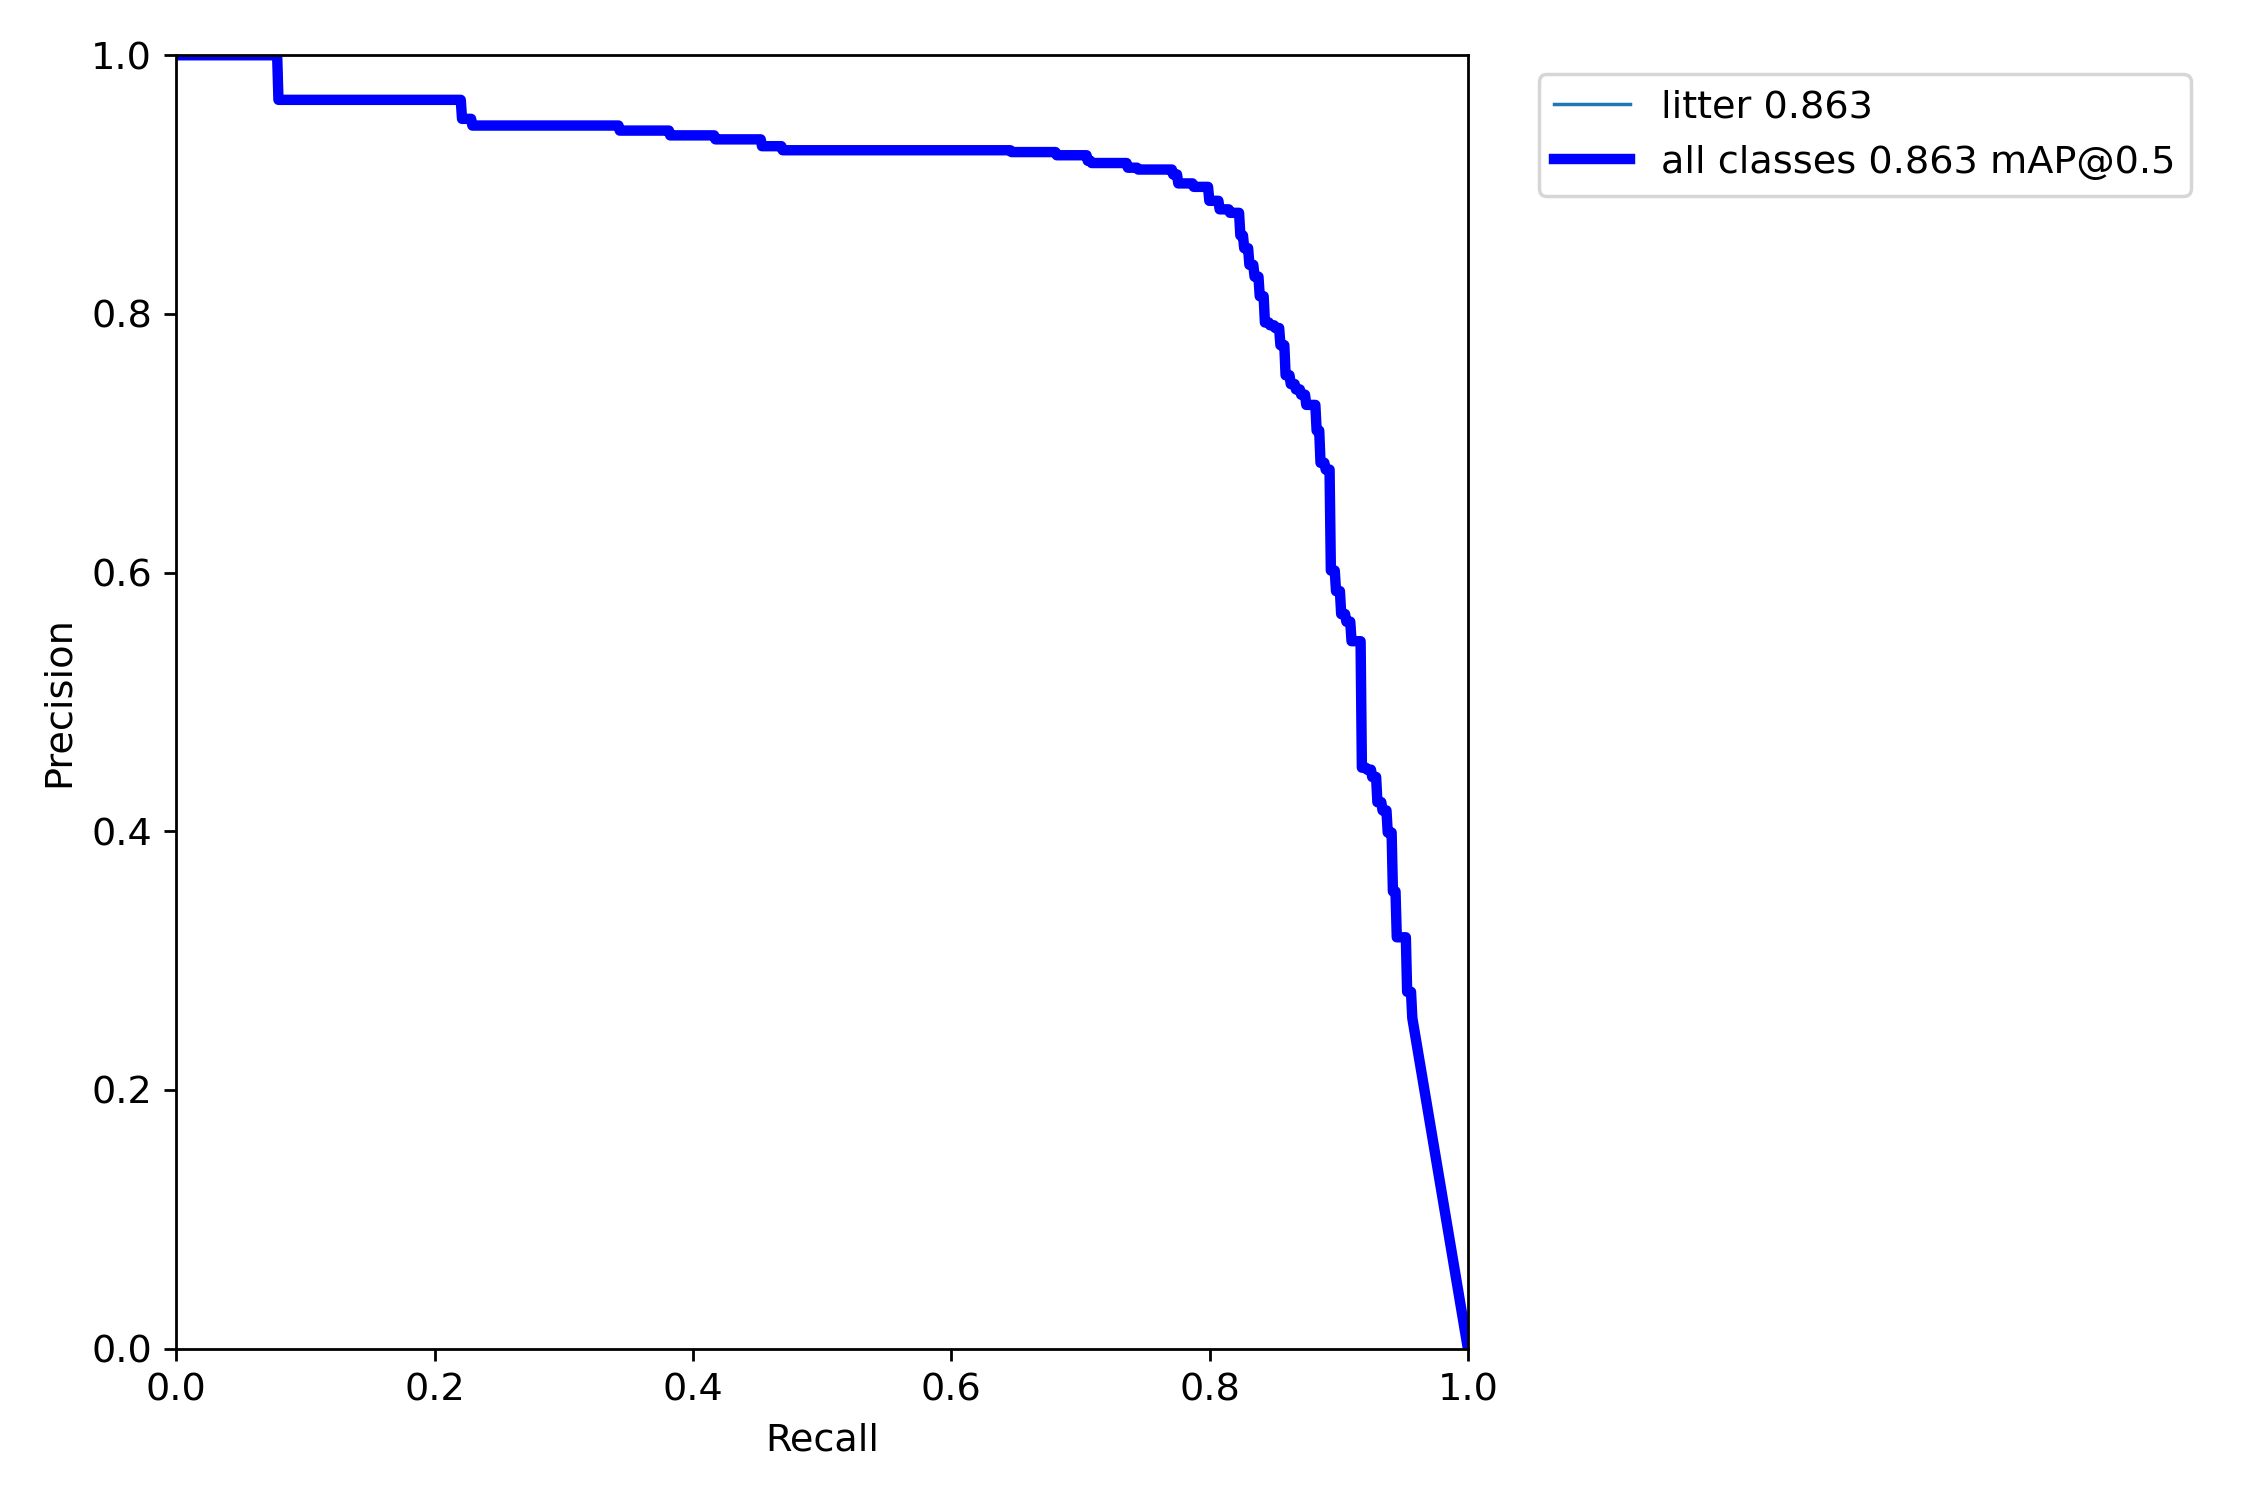
\includegraphics[scale=0.5]{images/fm-pr-curve.png}
    \caption{The precision-recall curve of the chosen model applied to the validation data.}
    \label{fig:fm-pr-curve}
\end{figure}

\begin{figure}[h!]
    \centering
    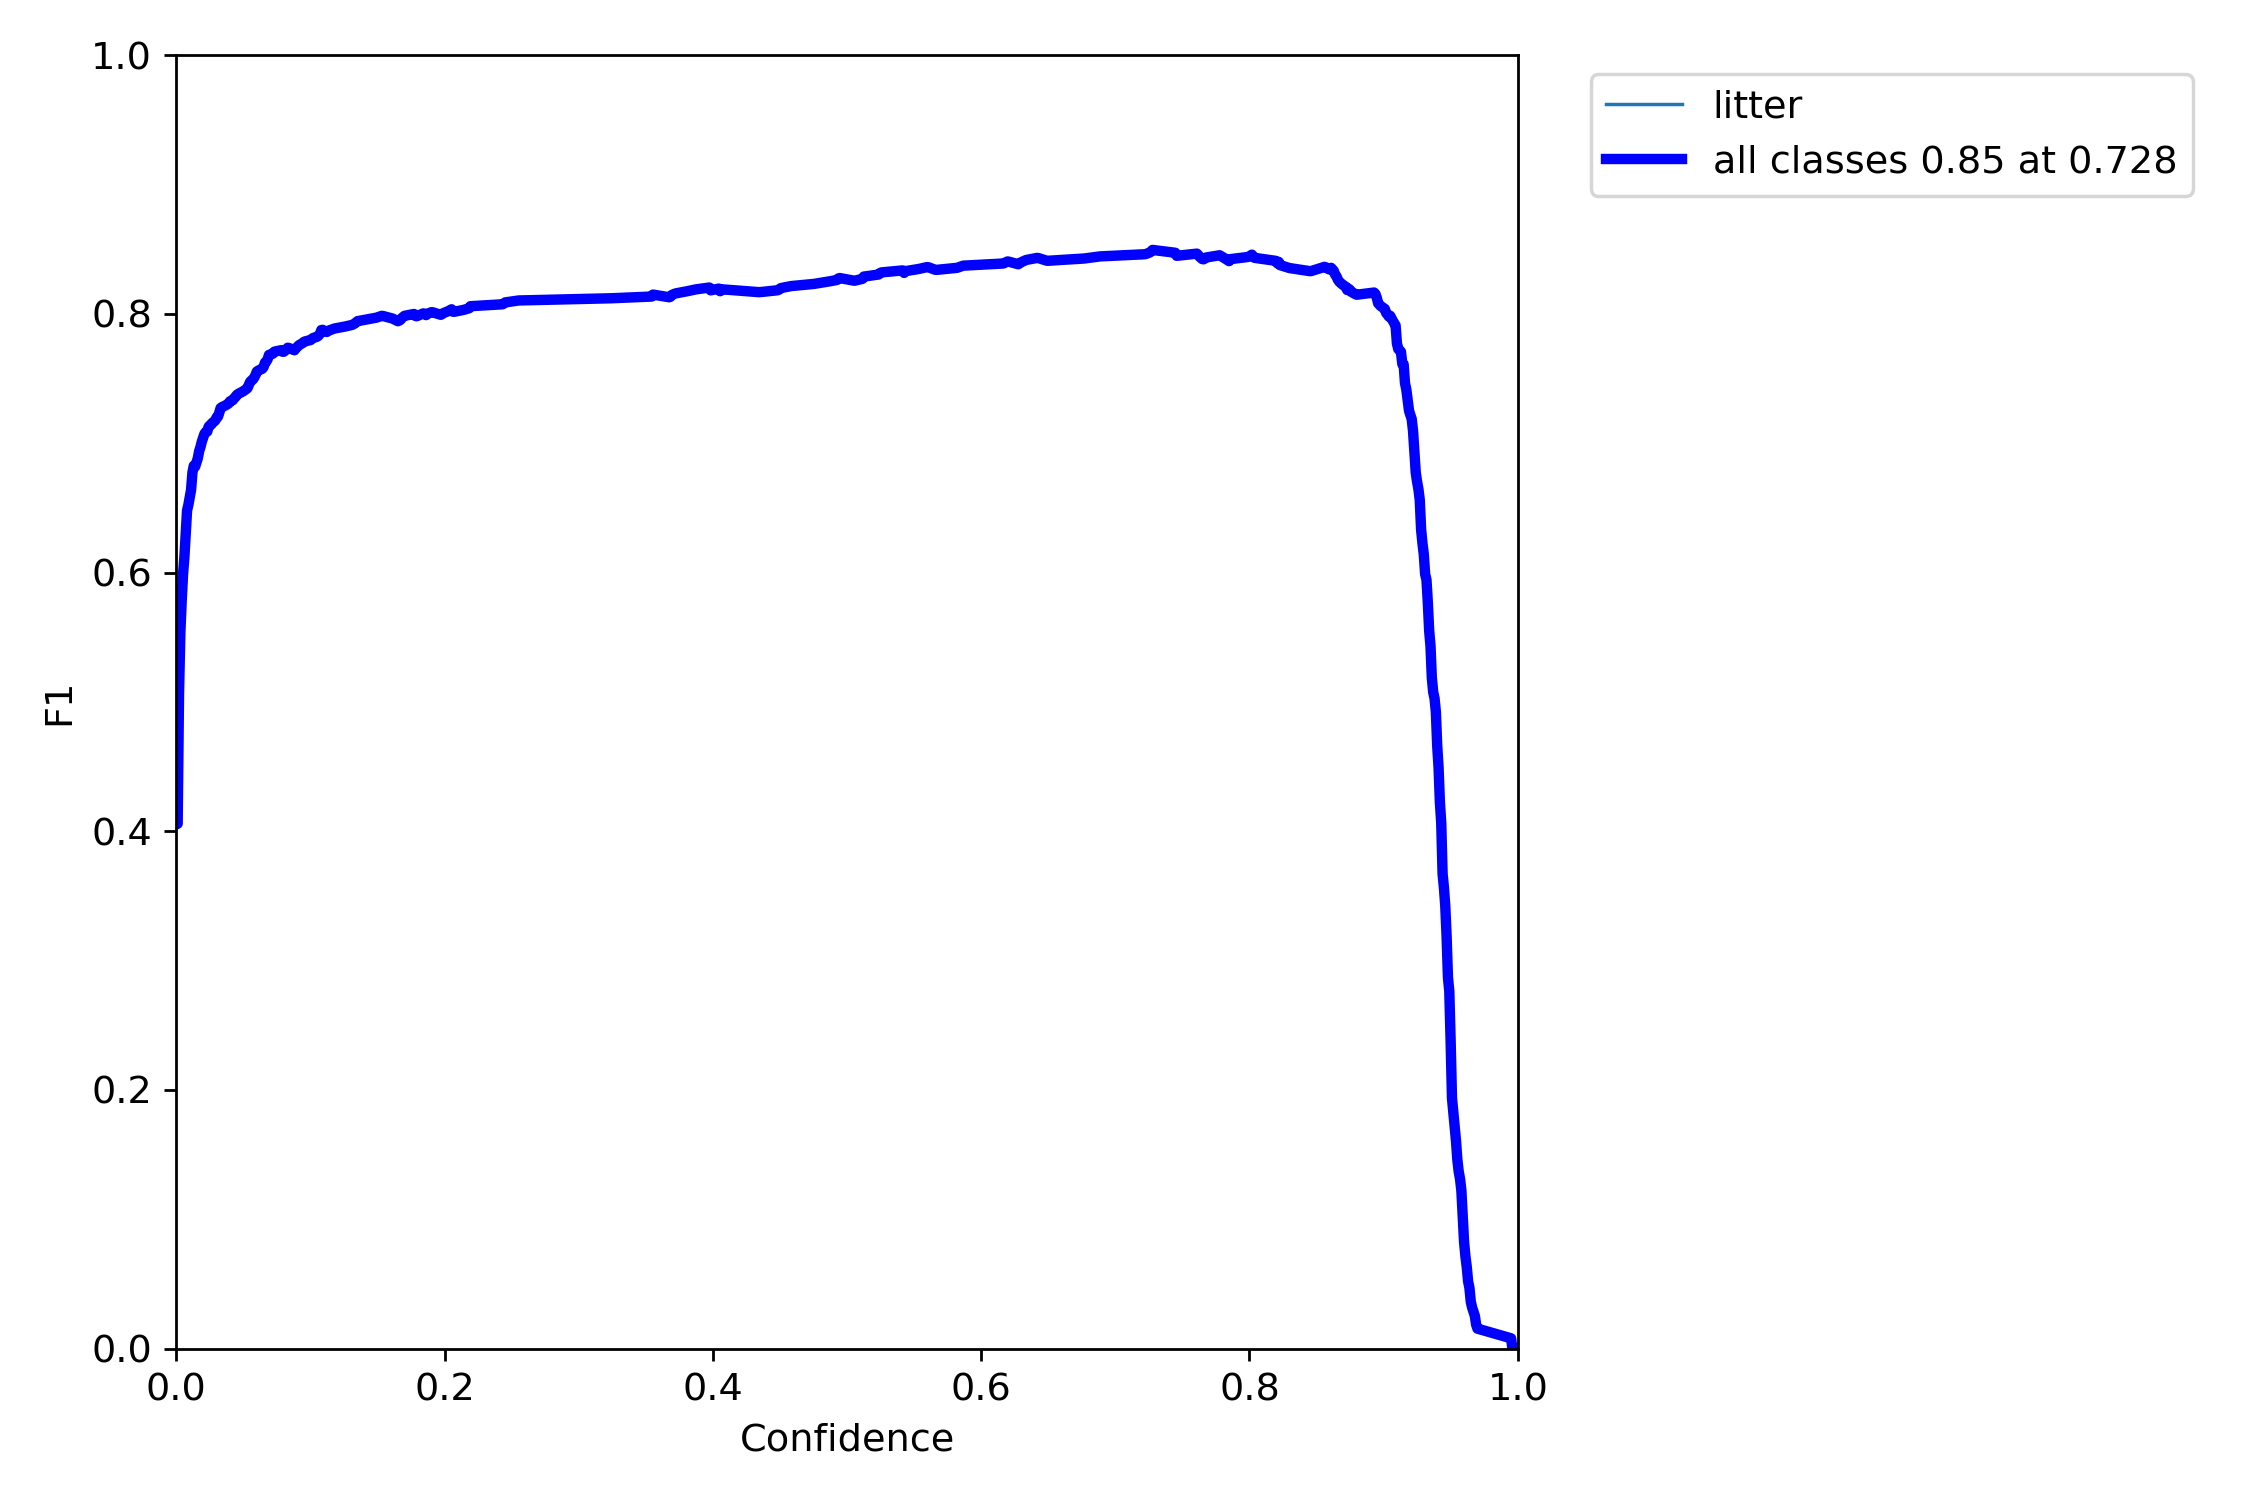
\includegraphics[scale=0.5]{images/fm-f1-curve.png}
    \caption{The F1 curve of the chosen model applied to the validation data.}
    \label{fig:fm-f1-curve}
\end{figure}

\begin{figure}[h]
    \centering
    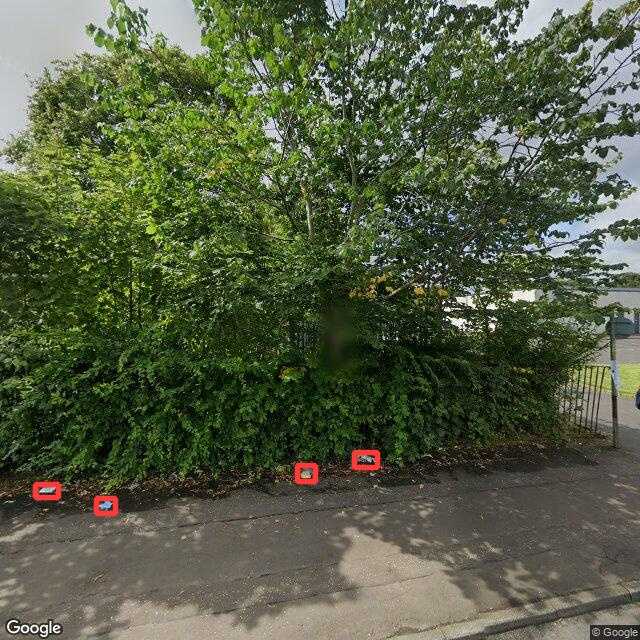
\includegraphics[scale=0.45]{images/good-4-in-bush.jpg}
    \caption{Four littered objects in a bush.}
    \label{fig:4-in-bush}
\end{figure}

\begin{figure}[h]
    \centering
    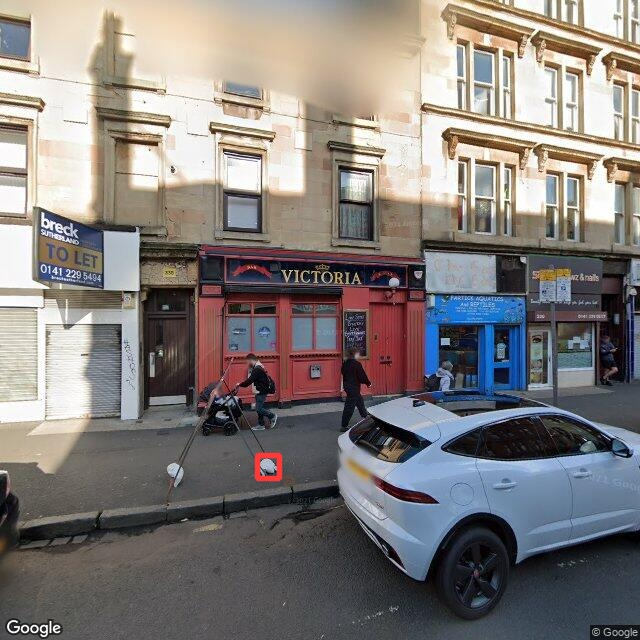
\includegraphics[scale=0.45]{images/flaw-sandbag.jpg}
    \caption{A white sandbag next to the kerb.}
    \label{fig:sandbag}
\end{figure}

\paragraph{Application To Glasgow City}

When applied to the 37,300 images collected within Glasgow City's data zones using a confidence threshold of 80\%, 7,732 litter objects were detected.

%\paragraph{Generalisation To Other Locations}

%For infrequent categories, the excessive over-sampling on them may cause severe over-fitting and degrade the generalisability of recognition on %these classes\cite{large-scale-object-detection}. 

\newpage
\section{Relationships}

Applying the final model to the test data produces the coefficients shown in Figure \ref{fig:nb-coeff-test}. The only potentially significant explanatory variable with a p-value less than .05 is \textit{no\_qualifications}. However, after applying Bonferroni Correction this is no longer the case and there are no significant predictors.

\begin{figure}[h]
    \centering
\footnotesize
\begin{verbatim}
                 Generalized Linear Model Regression Results                  
==============================================================================
Dep. Variable:                 litter   No. Observations:                   75
Model:                            GLM   Df Residuals:                       64
Model Family:        NegativeBinomial   Df Model:                           10
Link Function:                    Log   Scale:                          1.0000
Method:                          IRLS   Log-Likelihood:                -220.87
Date:                Mon, 14 Mar 2022   Deviance:                       44.777
Time:                        20:09:10   Pearson chi2:                     39.5
No. Iterations:                     7   Pseudo R-squ. (CS):             0.3903
Covariance Type:            nonrobust                                         
=====================================================================================
                        coef    std err          z      P>|z|      [0.025      0.975]
-------------------------------------------------------------------------------------
Intercept             2.1382      0.084     25.338      0.000       1.973       2.304
ALCOHOL               0.1139      0.185      0.615      0.539      -0.249       0.477
SMR                  -0.0124      0.110     -0.113      0.910      -0.229       0.204
Attainment            0.1627      0.152      1.071      0.284      -0.135       0.461
DEPRESS              -0.0593      0.182     -0.326      0.745      -0.416       0.298
EMERG                -0.3456      0.287     -1.204      0.229      -0.908       0.217
employment_rate       0.0701      0.395      0.177      0.859      -0.705       0.845
CIF                   0.0889      0.302      0.294      0.769      -0.504       0.681
Attendance           -0.0617      0.111     -0.556      0.578      -0.279       0.156
income_rate           0.0548      0.388      0.141      0.888      -0.705       0.814
no_qualifications     0.6634      0.236      2.806      0.005       0.200       1.127
=====================================================================================
\end{verbatim}
\normalsize
    \caption{The coefficients of the Negative Binomial regression model using the test data.}
    \label{fig:nb-coeff-test}
\end{figure}

The Pearson statistic is $\chi^2 = 39.5$ which is smaller than the $\chi^2(64)$ distribution, indicating that the model fits if the Negative Binomial is the correct model for the response. However, figure \ref{fig:predicted-vs-actual-test} shows that the wide residuals between the predicted and actual litter counts indicate that it does not perform very well.

\begin{figure}[h]
    \centering
    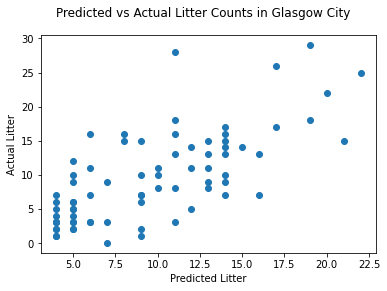
\includegraphics[scale=0.75]{images/predicted-vs-actual-test.png}
    \caption{The predicted litter counts vs the actual counts for the test data.}
    \label{fig:predicted-vs-actual-test}
\end{figure}

% Discussion ==================================================================

\chapter{Discussion}

\todo{Recommendations, Limitations and Future Work, Conclusion}

\section{Recommendations}

\section{Limitations and Future Work}

\subsection{Time and Hardware}



\section{Conclusion}

% Appendices ==================================================================

\begin{appendices}

\chapter{Detection Examples}

\begin{figure}[h]
    \centering
    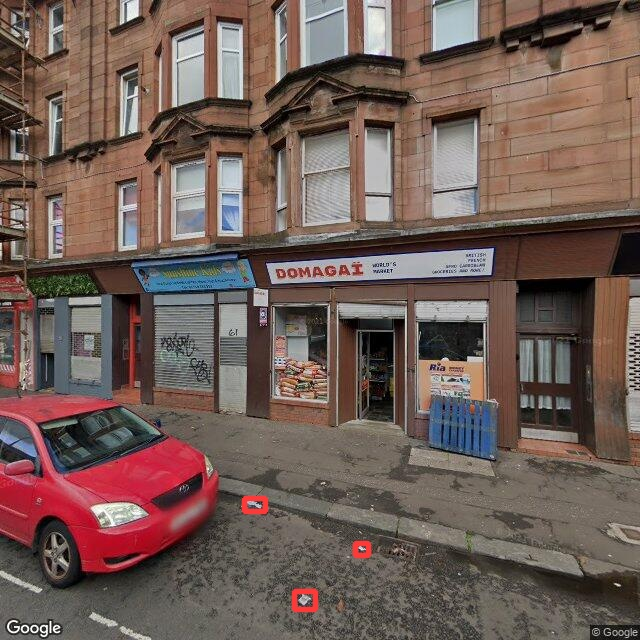
\includegraphics[scale=0.45]{images/good-three.jpg}
    \caption{A few littered objects next to the pavement.}
\end{figure}

\begin{figure}[h]
    \centering
    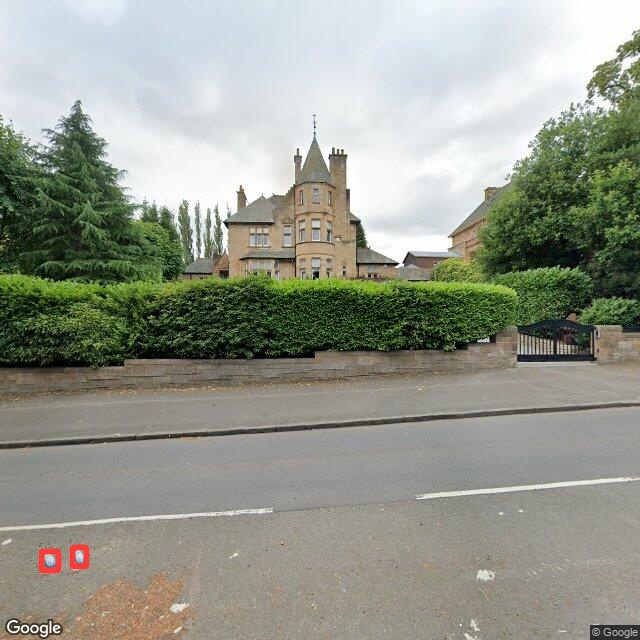
\includegraphics[scale=0.45]{images/good-two-bottles.jpg}
    \caption{Two plastic bottles on the road.}
\end{figure}

\begin{figure}[h]
    \centering
    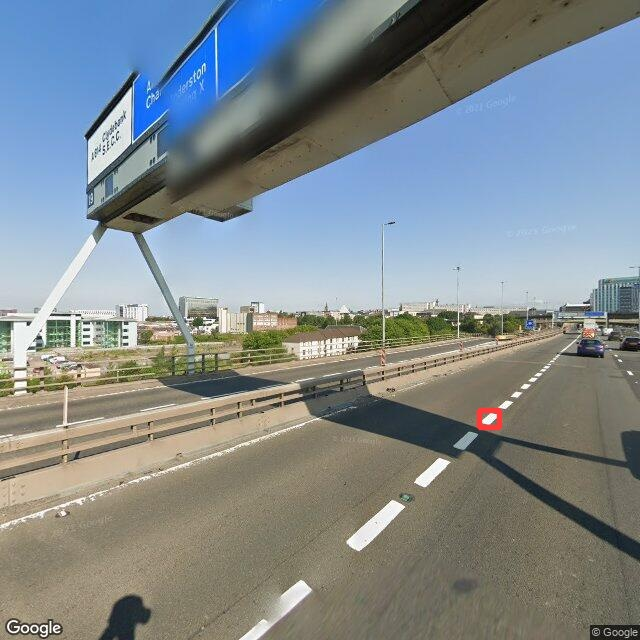
\includegraphics[scale=0.45]{images/flaw-road-marking.jpg}
    \caption{A white lane separator road marking.}
\end{figure}

\begin{figure}[h]
    \centering
    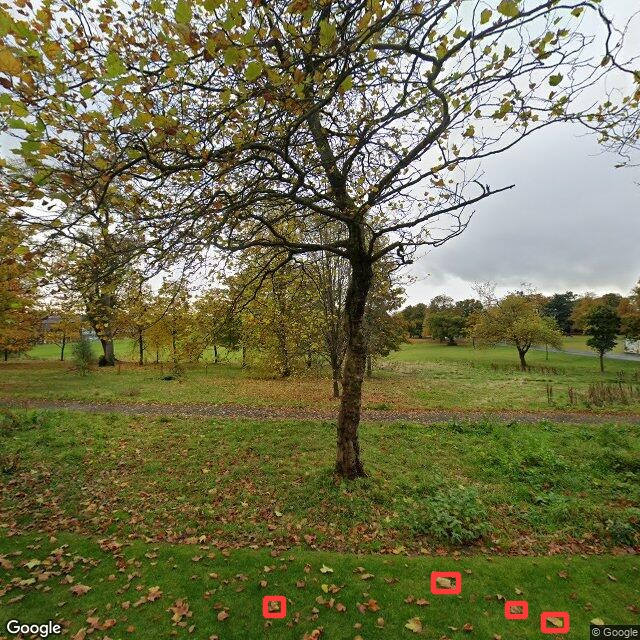
\includegraphics[scale=0.45]{images/flaw-tree-leaves.jpg}
    \caption{Leaves that have fallen from a nearby tree.}
\end{figure}

\end{appendices}

% Bibliography ================================================================

\bibliographystyle{abbrv}
\renewcommand{\thechapter}{0} % Don't number the bibliography
\bibliography{thesis}

\end{document}
